\section{User-centered Design Research}

\subsection{Mockup-Studie: Bewertung der Benutzerfreundlichkeit und
Funktionalität}
Bei der Entwicklung eines nutzerzentrierten Designs steht die direkte Einbindung
der Zielgruppe im Mittelpunkt. Dieser Ansatz, der als User-Centered Design (UCD) 
bezeichnet wird, stellt die Integration der Bedürfnisse, Erwartungen und
Anforderungen der Benutzer in den Entwicklungsprozess in den Mittelpunkt. Ziel
ist es, Produkte und Anwendungen zu gestalten, die nicht nur funktional und
ästhetisch ansprechend sind, sondern auch die bestmögliche
Benutzerfreundlichkeit bieten.

\subsubsection{Methodik und Teilnehmende}
Das in Kapitel \ref{sec:konzept} beschriebene Mockup des Studiengangsfinders wurde als Teil des UCD-Prozesses erarbeitet. Um sicherzustellen, dass das entworfene Konzept den Bedürfnissen der potenziellen Nutzer entspricht, wurde damit eine gezielte User-Centered-Design-Studie durchgeführt. Zu diesem Zweck wurden sechs Studierende und Absolventen verschiedener Fachrichtungen eingeladen, den Mockup-Entwurf zu evaluieren (siehe \autoref{table:teilnehmer-mockup-studie}).

\begin{table}[!ht]
    \centering
    \begin{tabular}{|l|l|l|l|}
        \hline
        \textbf{\#} & \textbf{Studienabschluss}                               & \textbf{Geschlecht} & \textbf{Datum} \\ \hline
        1           & Betriebswirtschaft B.A.                                 & Weiblich            & 16.09.2023     \\ \hline
        2           & Psychologie M.Sc.                                       & Weiblich            & 20.09.2023     \\ \hline
        3           & Informatik B.Sc.                                        & Männlich            & 25.09.2023     \\ \hline
        4           & Regenerative Energietechnik und Energieeffizienz B.Eng. & Männlich            & 07.10.2023     \\ \hline
        5           & Bioprozessinformatik B.Sc.                              & Männlich            & 08.10.2023     \\ \hline
        6           & Betriebswirtschaft B.A.                                 & Weiblich            & 12.10.2023     \\ \hline
    \end{tabular}

    \caption{Probanden der Mockup-Studie}
    \label{table:teilnehmer-mockup-studie}
\end{table}

\subsubsection{Ablauf des Tests}
Die Studie wurde in Form von Einzelinterviews durchgeführt. Die Teilnehmer wurden ermutigt, ihre persönlichen Perspektiven, Erfahrungen und Vorschläge einzubringen. Außerdem wurden sie gebeten, ihre Gedanken zum Entwurf laut zu äußern. Anschließend wurden ihnen nacheinander alle Grafiken des Entwurfs gezeigt (1. \autoref{fig:mockup-bubbles},
2. \autoref{fig:mockup-bubbles-hover}, 3. \autoref{fig:mockup-bubbles-popup}). 

Offene Fragen zu Designelementen, Verständlichkeit von Informationen und allgemeinen Nutzererfahrungen sollten Aufschluss über mögliche Stärken und Schwächen des Design-Proto\-typs geben. Ziel war es, frühzeitig wertvolles Feedback zu erhalten, um Optimierungen und Anpassungen vornehmen zu können, bevor die Umsetzung in die nächste Phase geht. Die lauten Gedanken der Teilnehmerinnen und Teilnehmer wurden von Herrn Huber in einem Freitextfeld dokumentiert.

\subsubsection{Ergebnisse der Mockup-Studie}
Die Ergebnisse der Mockup-Konzeptstudie sind Gegenstand der Diskussion und Interpretation in den folgenden Unterabschnitten. Die Rückmeldungen der Teilnehmerinnen und Teilnehmer an der Studie lassen sich zu konsistenten Mustern zusammenfassen, die in Rückmeldungen zu Bild 1, zu Bild 2, zu Bild 3 und in generelle Anmerkungen gruppiert wurden.

\paragraph{Bild 1: Visualisierung der Studiengänge}\label{sec:visualisierung-der-studiengänge}
Die Übersichtskarte wurde von den Teilnehmenden als unübersichtlich und geclustert wahrgenommen. Besonders die Farbähnlichkeit der Studiengänge wurde als störend
empfunden.

Eine konkrete Verbesserungsmöglichkeit besteht darin, die Überschriften der Nebel zu vergrößern und fett darzustellen, um die Lesbarkeit zu verbessern. Darüber hinaus wurde vorgeschlagen, alle Abkürzungen der Studiengänge standardmäßig auszublenden und nur den Nebel zu beschriften, um die Übersichtlichkeit zu erhöhen. Sobald der Benutzer mit der Maus in die Nähe des Nebels kommt, sollte die Überschrift des Nebels ausgeblendet und die Abkürzungen aller darin enthaltenen Studiengänge eingeblendet werden. Um die Zufälligkeit und Ähnlichkeit der Farben zu vermeiden, könnten die Studiengänge in den Fakultätsfarben und der Nebel im Hintergrund neutral (z.B. grau) eingefärbt werden.

\paragraph{Bild 2: Interaktivität}
Das Hover-Event über eine Bubble mit einem Tooltip wurde durchweg als passend und verständlich betrachtet. Dieses Element wurde von den Teilnehmenden als intuitiv und funktional empfunden.

\paragraph{Bild 3: Popup mit Details eines Studiengangs}
In Bezug auf die Anordnung der Informationen in dem Popup waren die Meinungen geteilt. Während einige eine absteigende Sortierung nach Relevanz bevorzugten, sprachen sich andere für eine alphabetische Sortierung aus. Die Auflistung ähnlicher Studiengänge wurde positiv bewertet. Die Darstellung der Branchen wurde als weniger aussagekräftig empfunden und teilweise vorgeschlagen, diese Information zu entfernen. Die Möglichkeit, sich Unternehmen in Regensburg anzeigen zu lassen, wurde positiv bewertet und es wurde angeregt, diese Funktion ausklappbar zu gestalten, um die Übersichtlichkeit zu erhöhen. Es wurde außerdem empfohlen, die Informationen zu den Einstiegsgehältern zu erläutern, möglicherweise durch die Integration von Fragezeichensymbolen und Tooltips.

\paragraph{Generelle Anmerkungen}
Zu den allgemeinen Verbesserungsvorschlägen gehören ein besserer Farbkontrast, mehr Erläuterungen zu verschiedenen Informationen und eine einheitliche und intuitive Anordnung der Designelemente, um die Übersichtlichkeit insgesamt zu erhöhen.

%
%
%
%
%
%
% PROTOTYPEN STUDIE
\subsection{Prototypen-Studie: Evaluation durch Studieninteressierte}
Basierend auf dem Mockup und den Erkenntnissen aus der Mockup-Studie wurde ein Prototyp entwickelt. Im Rahmen einer weiteren Studie wurden Studieninteressierte zum Testen des Prototyps von StudyMap eingeladen. Die Teilnehmer wurden gebeten, nach der selbstständigen Interaktion mit dem Prototypen an einer Umfrage teilzunehmen, um ihre Erfahrungen, Meinungen und Verbesserungsvorschläge zu dokumentieren.

Der folgende Abschnitt beleuchtet die Methodik, den genauen Ablauf des Tests und stellt die Ergebnisse dieser Evaluationsstudie vor, die wertvolle Einblicke in die Effektivität und Benutzerfreundlichkeit des Prototyps liefert.

\subsubsection{Methodik und Teilnehmende}
Der nächste Schritt im UCD-Prozess ist das Testen des Prototyps mit potenziellen Nutzern, d.h. Studieninteressierten. Zu diesem Zweck wurde auf der Grundlage des Mockups und der im vorherigen Kapitel beschriebenen Mockup-Studie ein Prototyp entwickelt (siehe \autoref{fig:prototyp-overview}). Ziel dieser Studie ist es, frühe Designentscheidungen zu hinterfragen und das Tool auf Usability zu testen. Der Vorteil einer solch frühen Evaluierung ist, dass größere Änderungen am Endprodukt wesentlich aufwendiger sind als in einem frühen Entwicklungsstadium.

\begin{figure}[H]
    \centering
    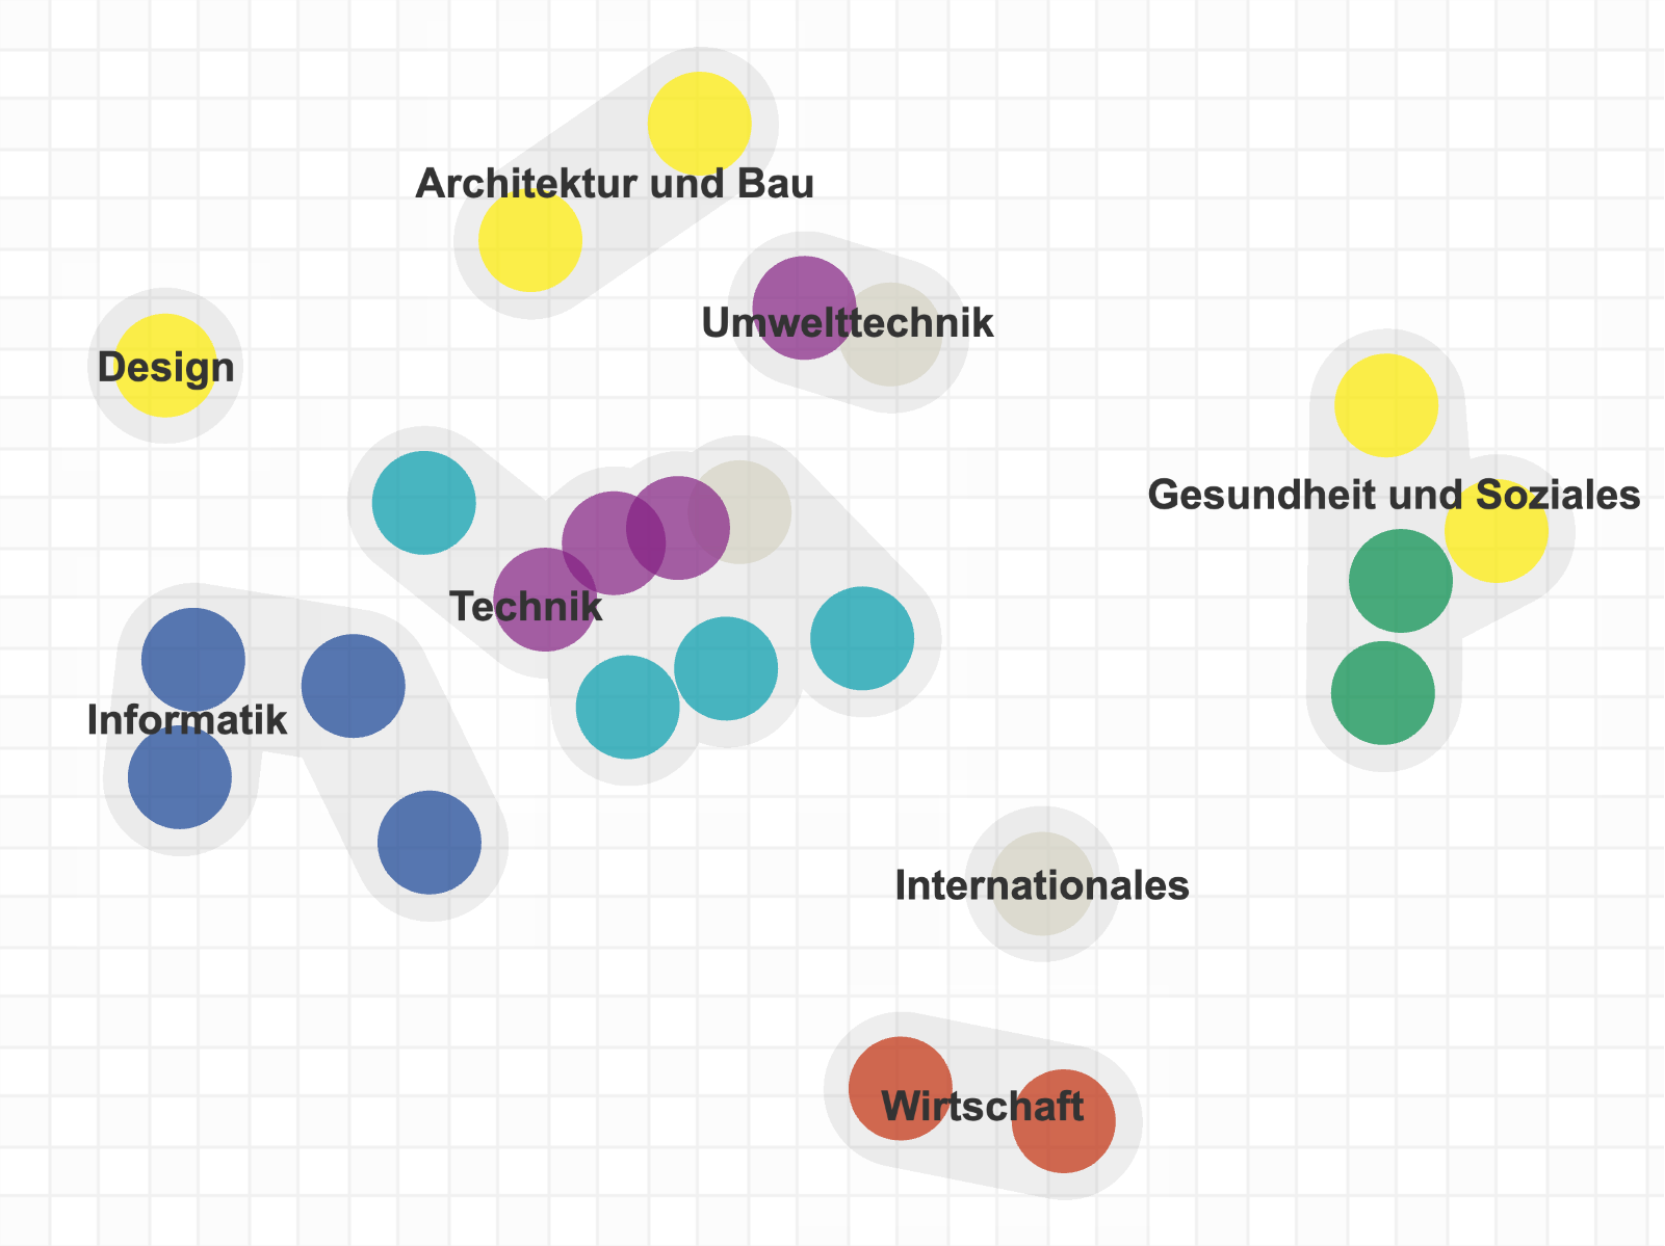
\includegraphics[width=\textwidth]{prototyp_overview}
    \caption{StudyMap Prototyp}
    \bildquelle{Eigene Darstellung}
    \label{fig:prototyp-overview}
\end{figure}

An der Studie nahmen 40 Schülerinnen und Schüler der 11. Klasse des Johannes-Nepomuk-Gymnasiums in Rohr i.NB teil. Alle diese Schüler werden voraussichtlich im Jahr 2026 die allgemeine Hochschulreife erlangen und entsprechen damit genau der Zielgruppe eines Studiengangfinders. Durch die örtliche Nähe des Gymnasiums zur OTH-Regensburg ist die Eignung des Teilnehmerkreises zusätzlich gegeben.

Die Befragung fand in zwei Gruppen (Klasse 11A und Klasse 11B) im Johannes-Neopomuk-Gymnasium vor Ort im Computerraum der Schule statt. Dort konnten die Schülerinnen und Schüler an den Windows-Rechnern der Schule sowohl den Prototyp testen als auch die Umfrage in Einzelarbeit beantworten.

\subsubsection{Ablauf des Tests}
Die Studie begann mit einer kurzen Einführung, in der den Teilnehmenden der
Zweck der Studie und die Handhabung des Prototyps erläutert wurden. Anschließend
wurden die Teilnehmenden gebeten, den Prototyp selbst zu verwenden und zwei
Aufgaben innerhalb einer Online-Umfrage zu lösen, um die Benutzerfreundlichkeit, die Navigationsstruktur und
die Funktionalitäten des Studiengangsfinders zu testen (siehe
\autoref{fig:prototyp-umfrage-aufgaben} - \textbf{Umfrage Teil 2}). In dieser Phase wurden sowohl
quantitative als auch qualitative Daten erhoben, um ein umfassendes Bild der 
Benutzererfahrung zu erhalten.

\begin{figure}[H]
    \centering
    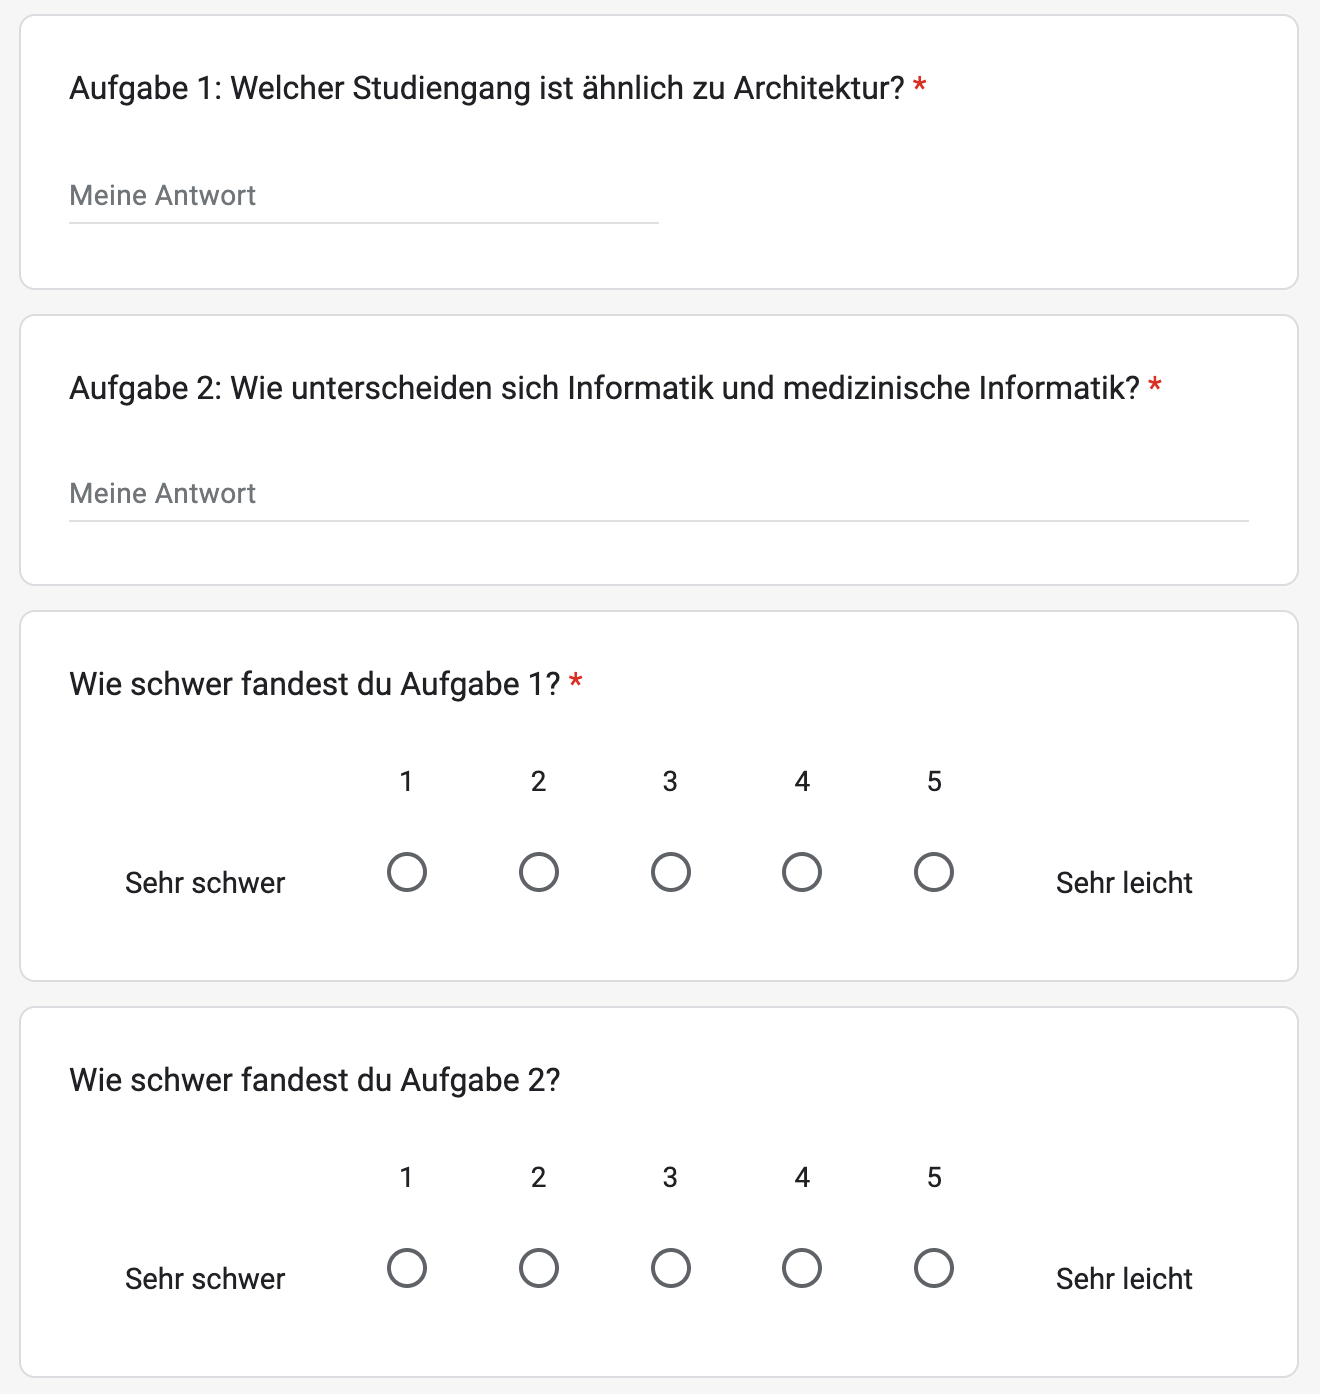
\includegraphics[width=0.5\textwidth]{umfrage_aufgaben}
    \caption{Prototypen-Studie: Aufgaben (Umfrage Teil 2)}
    \bildquelle{Eigene Darstellung}
    \label{fig:prototyp-umfrage-aufgaben}
\end{figure}

Nach der Interaktion mit dem Prototyp wurden die Teilnehmenden gebeten, zusätzlich zu den Aufgaben weitere Fragen in der anonymen Online-Umfrage zu beantworten.

Die ersten Fragen der Umfrage waren Multiple-Choice-Fragen mit den Antwortmöglichkeiten \glqq Ja\grqq{}, \glqq Nein\grqq{} und \glqq Keine Angabe\grqq{} \textbf{(Umfrage Teil 1)}.

\begin{enumerate}
    \item Willst du nach dem Abi studieren?
    \item Wenn ja, weißt du schon, was für ein Studium?
    \item Würde dir StudyMap bei der Wahl des Studiengangs helfen?
    \item Die Antwort hier ist \glqq Ja\grqq{} (Aufmerksamkeitsfrage)
\end{enumerate}

Danach folgten die beiden oben beschriebenen Aufgaben (siehe
\autoref{fig:prototyp-umfrage-aufgaben}). Zuletzt wurden die folgenden Fragen
mit Freitextfeldern zur Beantwortung gestellt \textbf{(Umfrage Teil 3)}:

\begin{enumerate}
    \item Was findest du an dem Konzept gut?
    \item Was findest du am Konzept schlecht?
    \item Hast du neue Ideen für den Prototyp?
    \item Wenn du bei \glqq Würde StudyMap dir bei der Studienwahl helfen?\grqq{} NEIN angekreuzt hast: Warum nicht?
\end{enumerate}

Die Fragen wurden bewusst mit Freitextfeldern zur Beantwortung versehen, um den Teilnehmenden die Möglichkeit zu geben, mit allen möglichen Gedankengängen zu antworten. Dies kann dazu führen, dass Ideen entstehen, die bisher noch nicht bedacht wurden und somit im Endprodukt umgesetzt werden können. Die Befragung dauerte ca. 15 Minuten. Durch die Kombination der Interaktion mit dem Prototyp und der schriftlichen Befragung konnten vielfältige Einblicke in die Nutzerperspektive gewonnen werden.

\subsubsection{Ergebnisse der Prototypen-Studie}

\paragraph{Umfrage Teil 1: Fragen}

\begin{figure}[H]
    \centering
    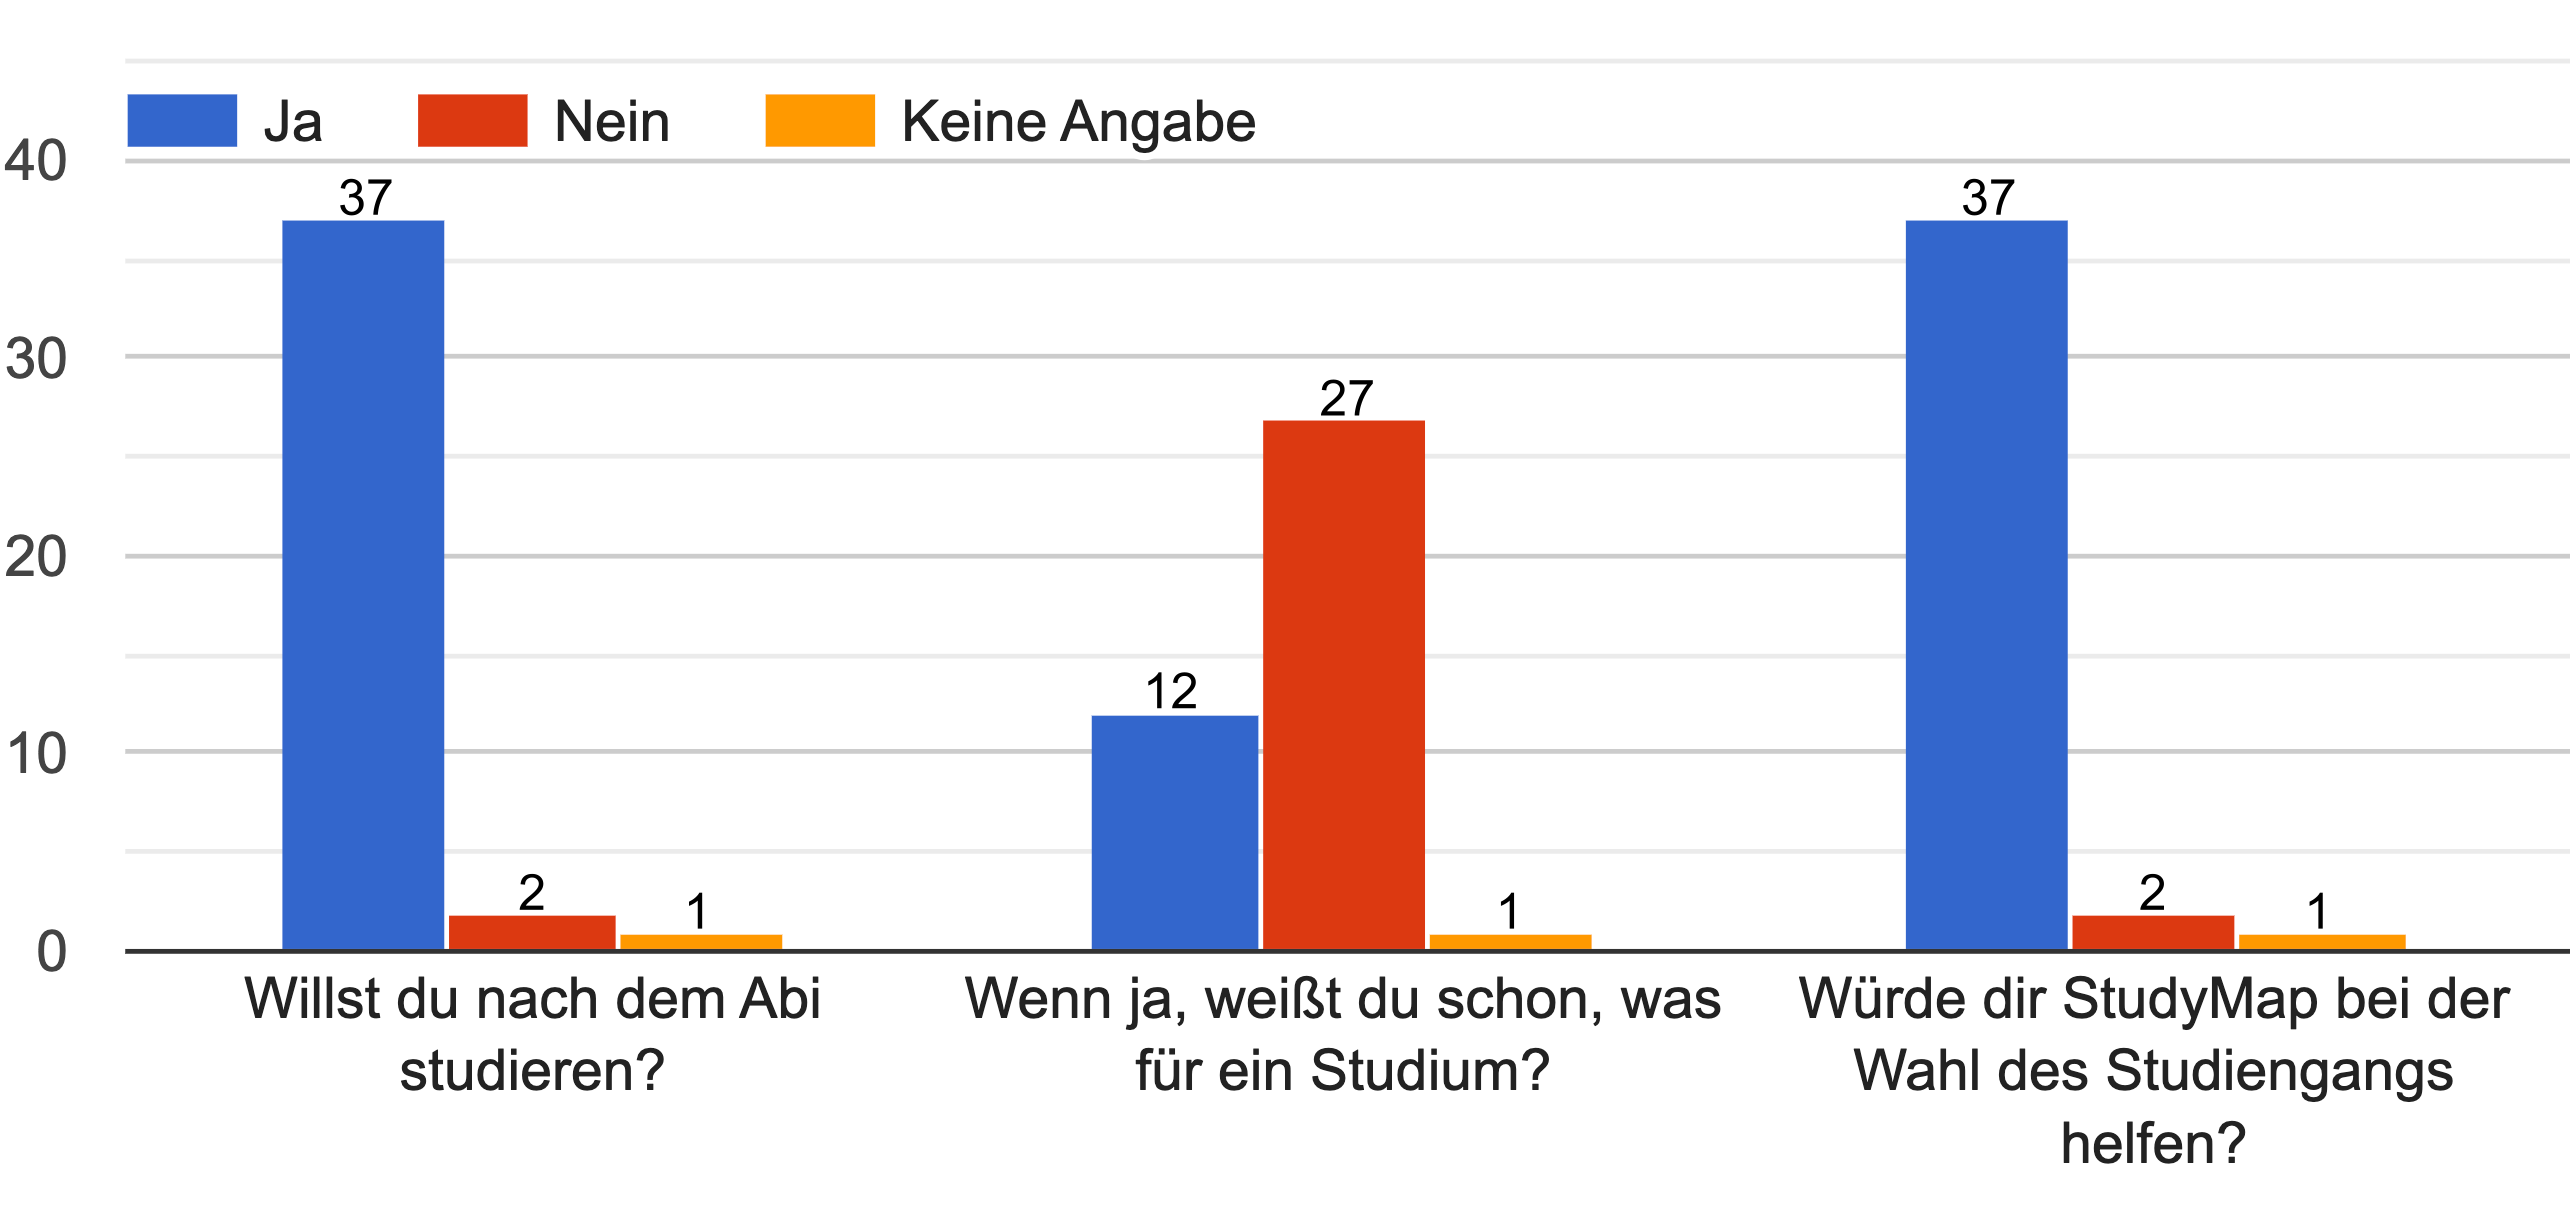
\includegraphics[width=\textwidth]{linien_fragen_1}
    \caption{Ergebnisse: Teil 1}
    \bildquelle{Google Forms + selbst ergänzte absolute Werte}
    \label{fig:linien-fragen-1}
\end{figure}

\autoref{fig:linien-fragen-1} zeigt, dass die erste Frage (\glqq Möchtest du nach dem Abitur studieren?\grqq{}) von 92,5 \% der Befragten bejaht wurde. Während zwei Personen (5 \%) die Frage verneinten, machte nur eine Person (2,5 \%) keine Angabe. Daraus lässt sich schließen, dass es sich bei der gewählten Teilnehmergruppe tatsächlich um die richtige Zielgruppe von StudyMap handelt.

Auf die Frage \glqq Wenn ja, weißt du schon, was du studieren willst?\grqq{} antworteten 30 \% (12) der Befragten mit \glqq Ja\grqq{}. 67,5 \% (27) haben mit \glqq Nein\grqq{} geantwortet und 2,5 \% haben wiederum die Angabe verweigert. Die Person, die bei Frage 1 angegeben hat, nicht zu antworten, hat bei dieser Frage mit \glqq Nein\grqq{} geantwortet. Die Person, die bei Frage 2 mit \glqq Keine Angabe\grqq{} stimmte, hatte zuvor bei Frage 1 mit \glqq Ja\grqq{} gestimmt. Die beiden Schüler, die bei Frage 1 mit \glqq Nein\grqq{} für ein Studium geantwortet haben, haben auch Frage 2 mit \glqq Nein\grqq{} votiert.

Zieht man die beiden Schülerinnen und Schüler, die sich bei Frage 1 gegen ein Studium entschieden haben, von den \glqq Nein\grqq{}-Antworten bei Frage 2 ab, so verbleiben 25 von 37 Studieninteressierten, die noch nicht wissen, was sie studieren werden. Daraus ergibt sich ein Anteil von 67,57 \% der Schüler der 11. Klasse, welche voraussichtlich nach dem Abitur eine Studienorientierung benötigen. Dieser Anteil an Schülern könnte mithilfe des innovativen Studiengangsfinders zu einem passenden Studiengang geführt werden.

Die dritte Frage (\glqq Würde dir StudyMap bei der Studienwahl helfen?\grqq{}) wurde von 37 von 40 Teilnehmern (92,5 \%) bejaht. Zwei Teilnehmer antworteten mit \glqq Nein\grqq{} und eine Person enthielt sich der Stimme. Im Falle einer Verneinung hatten die Befragten die Möglichkeit, dies im Anschluss in einem Freitextfeld zu begründen. Die beiden Personen, die mit \glqq Nein\grqq{} geantwortet haben, gaben an, dass StudyMap ihnen nicht bei der Studienwahl helfen würde, da sie bereits wüssten, was sie studieren wollen. Die Antworten auf diese Frage verdeutlichen noch einmal den Bedarf des Studiengangsfinders als Orientierungshilfe für Studieninteressierte.

Die Frage Nr. 4 der Umfrage Teil 1 wurde von allen Teilnehmern korrekt mit \glqq Ja\grqq{} beantwortet. Sie diente dazu, willkürlich ausgefüllte und damit nicht auswertbare Teilnahmen aus der Befragung auszusortieren.

\paragraph{Umfrage Teil 2: Aufgaben}

\begin{figure}[H]
    \centering
    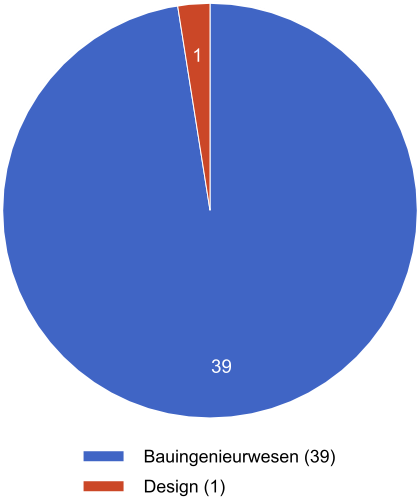
\includegraphics[width=0.4\textwidth]{torte_bauingenieur}
    \caption{Welcher Studiengang ist ähnlich zu Architektur? (Aufgabe 1)}
    \bildquelle{Eigene Darstellung}
    \label{fig:prototyp-umfrage-bauingenieur}
\end{figure}

In Aufgabe 1 sollten die Studienteilnehmer herausfinden, welcher Studiengang dem Studiengang "Architektur" ähnlich ist. Als Hilfsmittel stand ihnen der Live-Prototyp zur Verfügung. Wie in den vorherigen Kapiteln erläutert, werden ähnliche Studiengänge durch den MDS-Algorithmus nahe beieinander platziert. Die Lösung war daher der Studiengang \glqq Bauingenieurwesen\grqq{} (siehe \autoref{fig:prototyp-umfrage-bauingenieur-erklaerung}). 39 von 40 Studierenden (97,5 \%) lösten diese Aufgabe richtig. Die einzige falsche abgegebene Antwort entsprach dem Studiengang \glqq Design\grqq{}. \glqq Design\grqq{} ist im Prototyp eine Inhaltskategorie und kein Studiengang, ist aber tatsächlich dem Studiengang \glqq Architektur\grqq{} benachbart. Die hohe Übereinstimmung mit der Lösung weist auf die Intuitivität des Konzepts hin und stärkt damit die Basis für die weitere Entwicklung.

\begin{figure}[H]
    \centering
    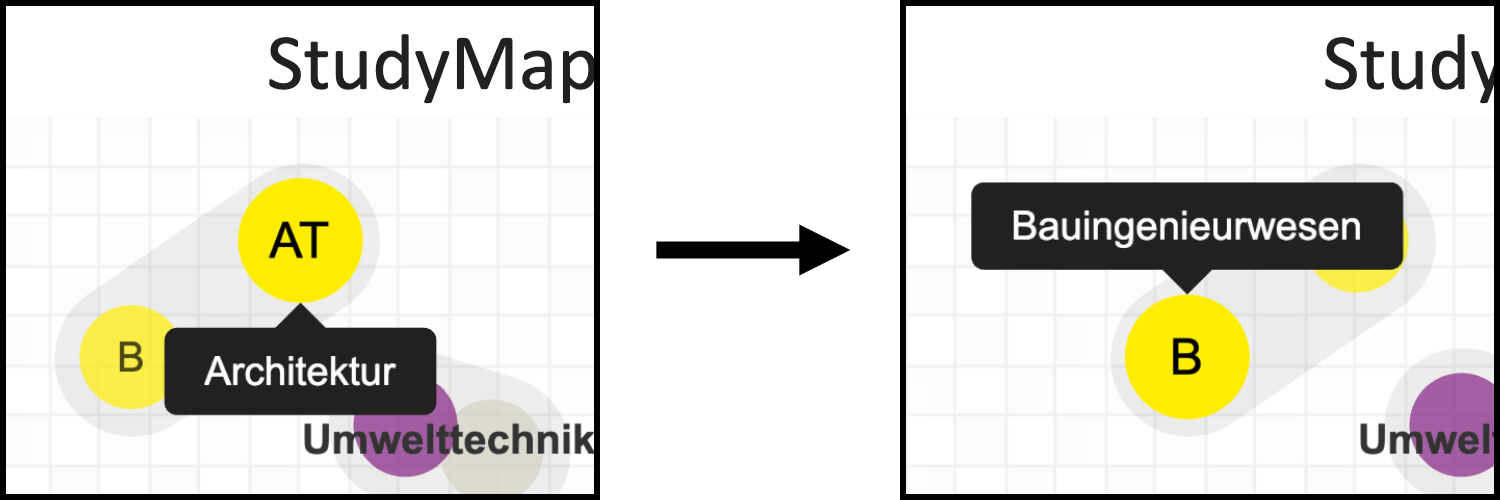
\includegraphics[width=0.65\textwidth]{prototyp_at_b}
    \caption{Prototyp: Architektur -> Bauingenieurwesen (Aufgabe 1)}
    \bildquelle{Eigene Darstellung}
    \label{fig:prototyp-umfrage-bauingenieur-erklaerung}
\end{figure}

%% Aufgabe 2
In der zweiten Aufgabe sollten die Studieninteressierten herausfinden, inwiefern sich die allgemeine Informatik vom Studiengang Medizinische Informatik unterscheidet. Testweise wurde ein Feature entwickelt und zum Prototyp hinzugefügt, das es ermöglicht, Studiengänge zu vergleichen, ohne das Popup mit den Studiengangdetails schließen und erneut öffnen zu müssen.

\begin{figure}[H]
    \centering
    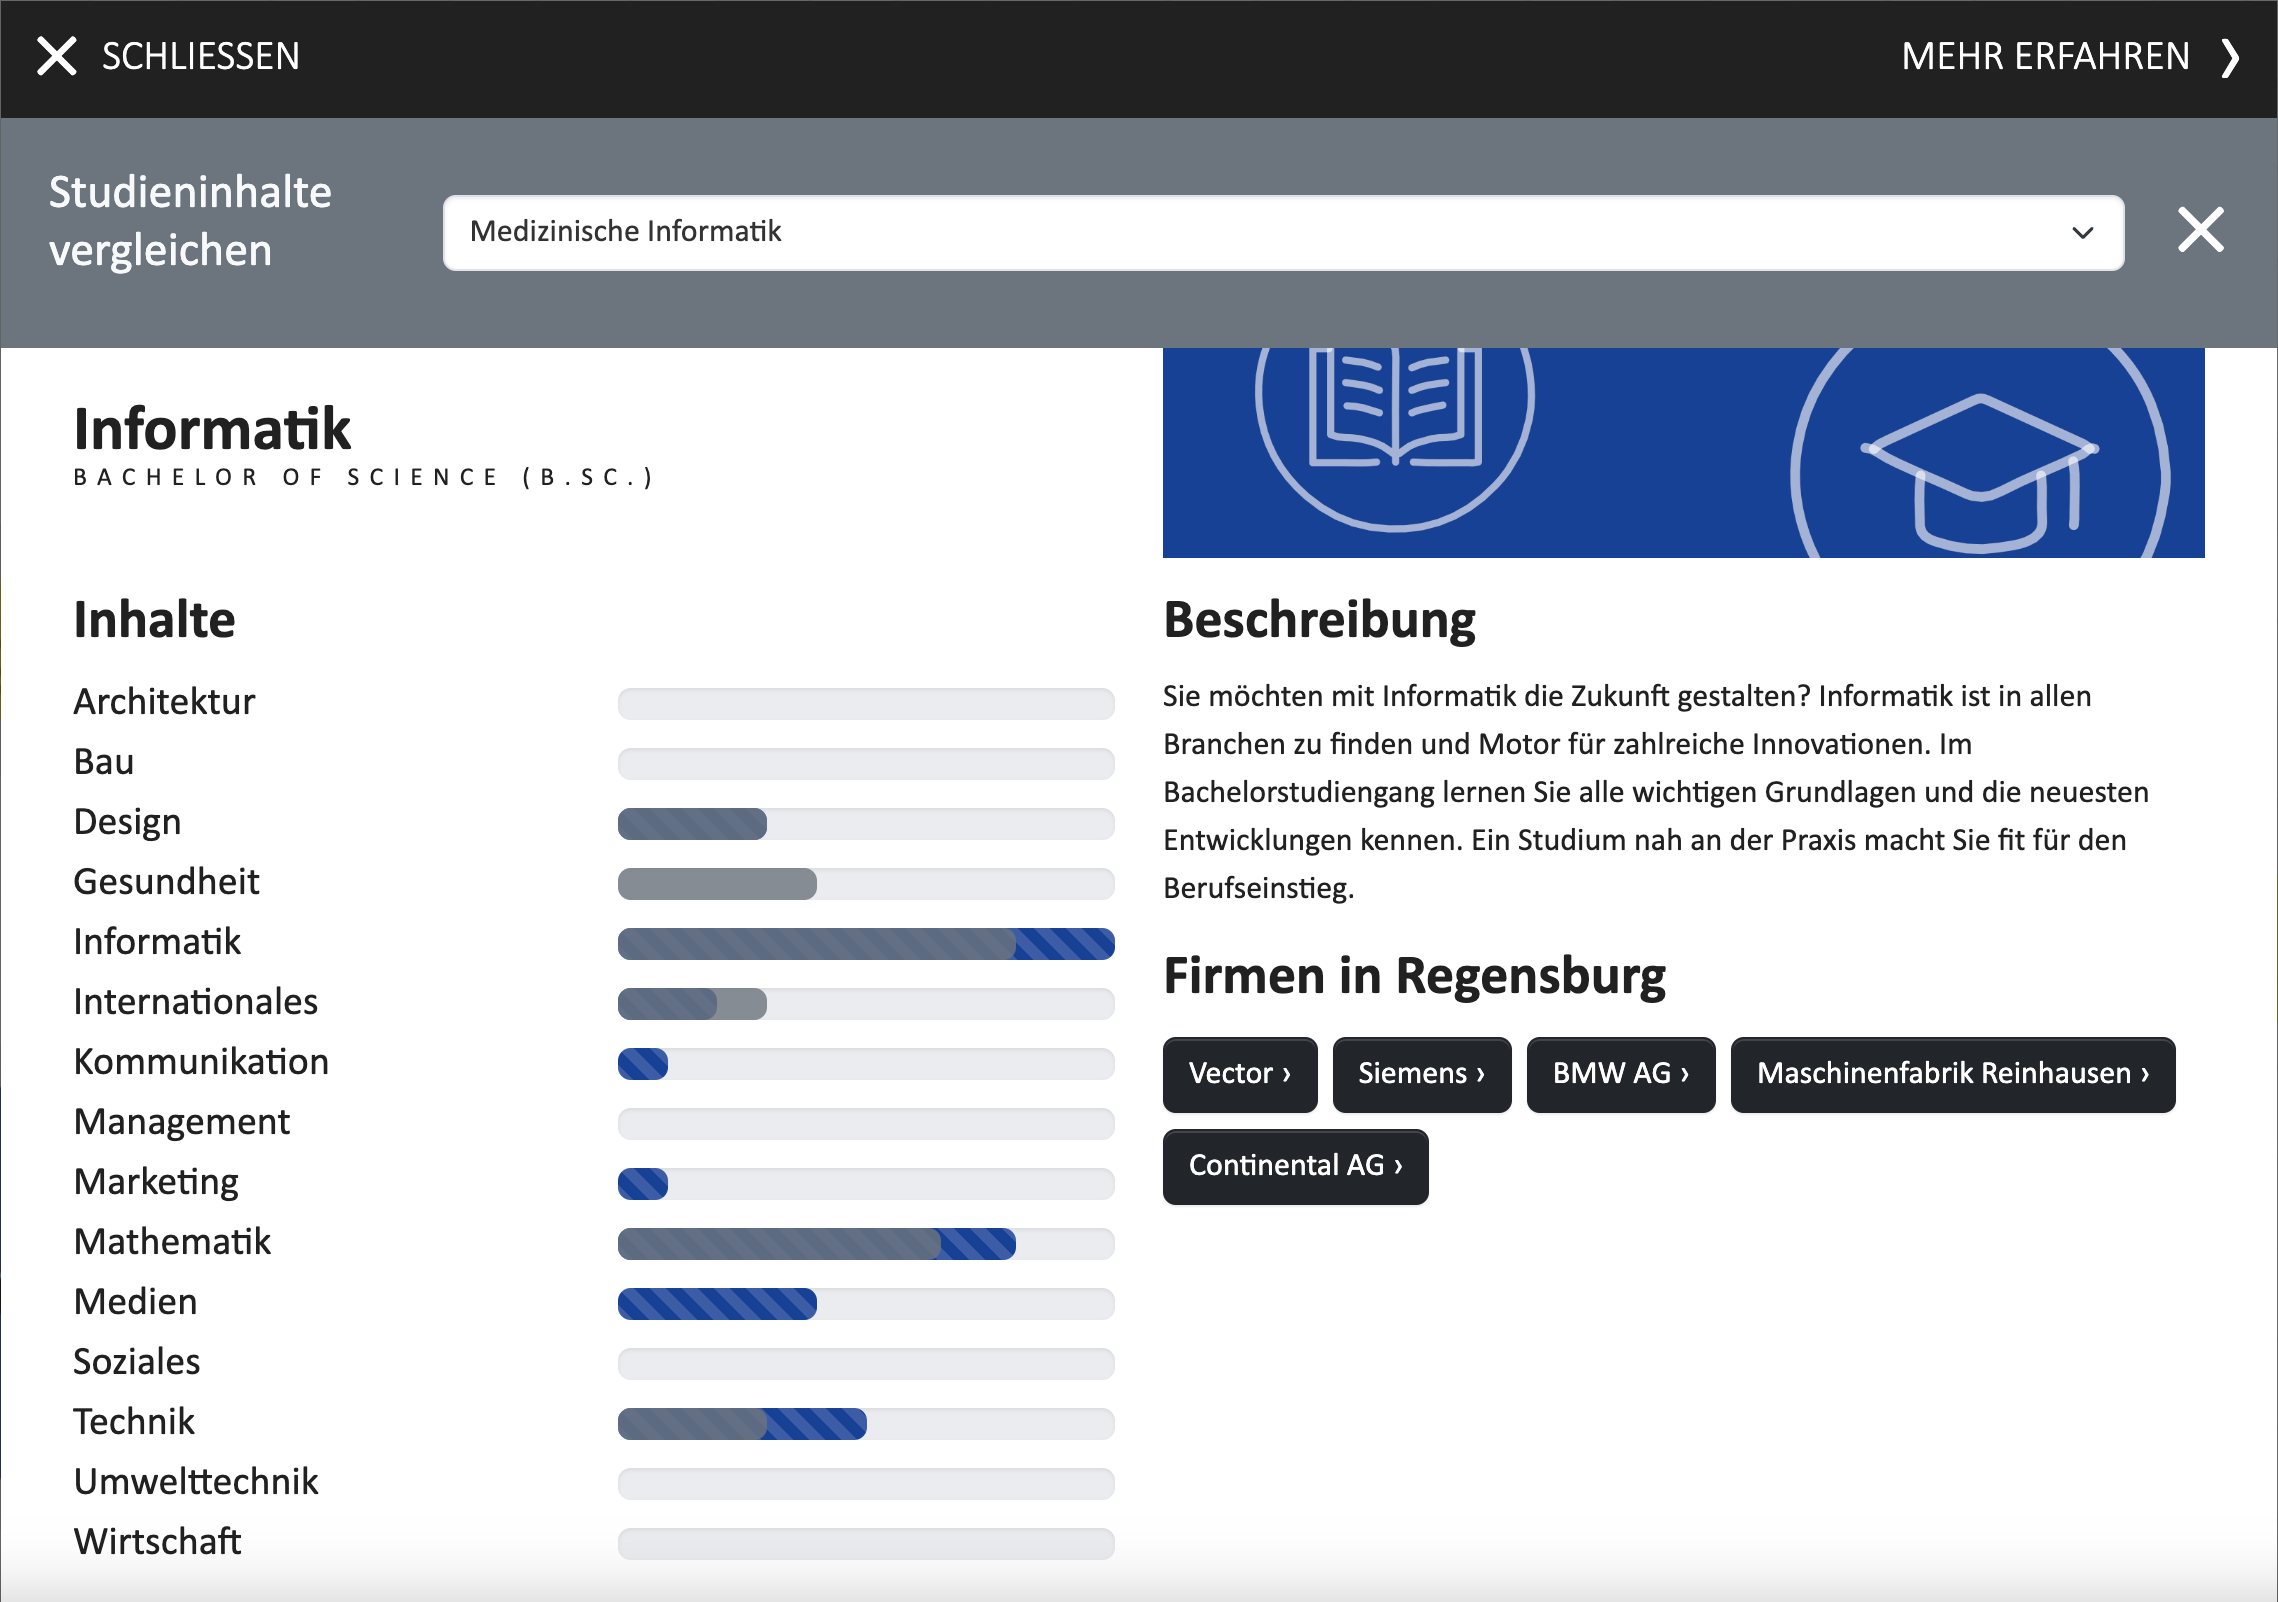
\includegraphics[width=0.8\textwidth]{prototyp_comparison_i_im}
    \caption{Prototyp: Vergleichsfeature}
    \bildquelle{Eigene Darstellung}
    \label{fig:prototyp-comparison}
\end{figure}

\autoref{fig:prototyp-comparison} zeigt den Vergleich der Studiengänge Informatik und Medizinische Informatik. Die farbigen Inhaltsbalken zeigen die Inhalte des ursprünglich ausgewählten Studiengangs an. Jeder Studiengang hat die Farbe seiner zugehörigen Fakultät. Wenn ein Studiengang zum Vergleich hinzugefügt wird, werden dessen Inhalte mit grauen Balken über die anderen Inhalten gelegt. Es ist wichtig, dass die Inhalte klar und verständlich dargestellt werden, ohne dabei subjektive Bewertungen einzubeziehen. Der Vergleich kann über das X-Symbol im grauen Balken gelöscht und eingeklappt werden.

\begin{figure}[H]
    \centering
    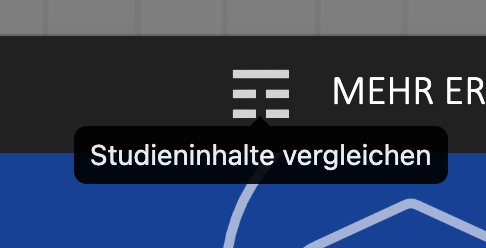
\includegraphics[width=0.3\textwidth]{prototyp_open_comparison}
    \caption{Prototyp: Vergleichsfeature öffnen}
    \bildquelle{Eigene Darstellung}
    \label{fig:prototyp-comparison-open}
\end{figure}

Die Schülerinnen und Schüler können mithilfe dieser Funktion die zweite Aufgabe bearbeiten. Wie in \autoref{fig:prototyp-comparison-open} gezeigt, kann das Feature über den mit einem Tooltip beschrifteten Knopf im Header des Popups ausgeklappt werden. Um zur Lösung zu gelangen, gibt es zwei Wege:

\begin{enumerate}
    \item Informatik-Bubble anklicken und mit Medizinische Informatik vergleichen
    \item \glqq Medizinische Informatik\grqq{}-Bubble anklicken und mit Informatik vergleichen
\end{enumerate}

Beides ergibt dasselbe Inhaltsdiagramm, aus dem sich die Unterschiede in den Studiengängen ablesen lassen.

Die Auswertung der Antworten auf Aufgabe 2 zeigt, dass die Mehrheit der Probanden das System und das Konzept hinter StudyMap verstanden hat. In \autoref{fig:prototyp-comparison-wordcloud} sind einige der genannten Schlagwörter in Form einer \textit{Wordcloud} dargestellt.

Eine Wordcloud ist eine grafische Darstellung von Textdaten. Dabei werden häufig vorkommende Wörter größer und prominenter dargestellt als seltener vorkommende Wörter. Sie bietet eine schnelle visuelle Zusammenfassung der wichtigsten Begriffe in einem Text oder einer Gruppe von Texten. Außerdem dient sie dazu, einen Überblick über die Antworten zu geben, ohne alle ausformulierten Antworten zu enthalten.

Die Begriffe \textit{Gesundheit}, \textit{Informatik}, \textit{Mathematik}, \textit{Internationales} und \textit{Medien} sind sehr prominent (siehe \autoref{fig:prototyp-comparison-wordcloud}). Da diese Begriffe die inhaltlichen Kategorien im Prototyp repräsentieren und sich die Werte in den beiden Studiengängen unterscheiden, sind sie die richtigen Antworten für die Aufgabe. Daher kann die anfänglich genannte These, dass das Konzept verstanden wurde, bestätigt werden. Die Antworten der Teilnehmenden sind im Anhang ausformuliert vorzufinden.

\begin{figure}[H]
    \centering
    
\includegraphics[width=0.6\textwidth]{aufgabe2-wordcloud}
    \caption{Wordcloud der Antworten (Aufgabe 2)}
    \bildquelle{Eigene Darstellung}
    \label{fig:prototyp-comparison-wordcloud}
\end{figure}

% Später
% Schwierigkeit
Anschließend an die beiden Aufgaben wurden die Teilnehmer nach ihrer Schwierigkeitsbeurteilung befragt. Die Schüler und Schülerinnen bewerteten jeweils die Aufgaben von 1 bis 5 (1: sehr schwer, 5: sehr leicht). Anhand der folgenden \autoref{fig:prototyp-umfrage-aufgabe-1-schwierigkeit} ist erkennbar, dass die meisten Teilnehmer Aufgabe 1 als einfach empfanden.

\begin{figure}[H]
    \centering
    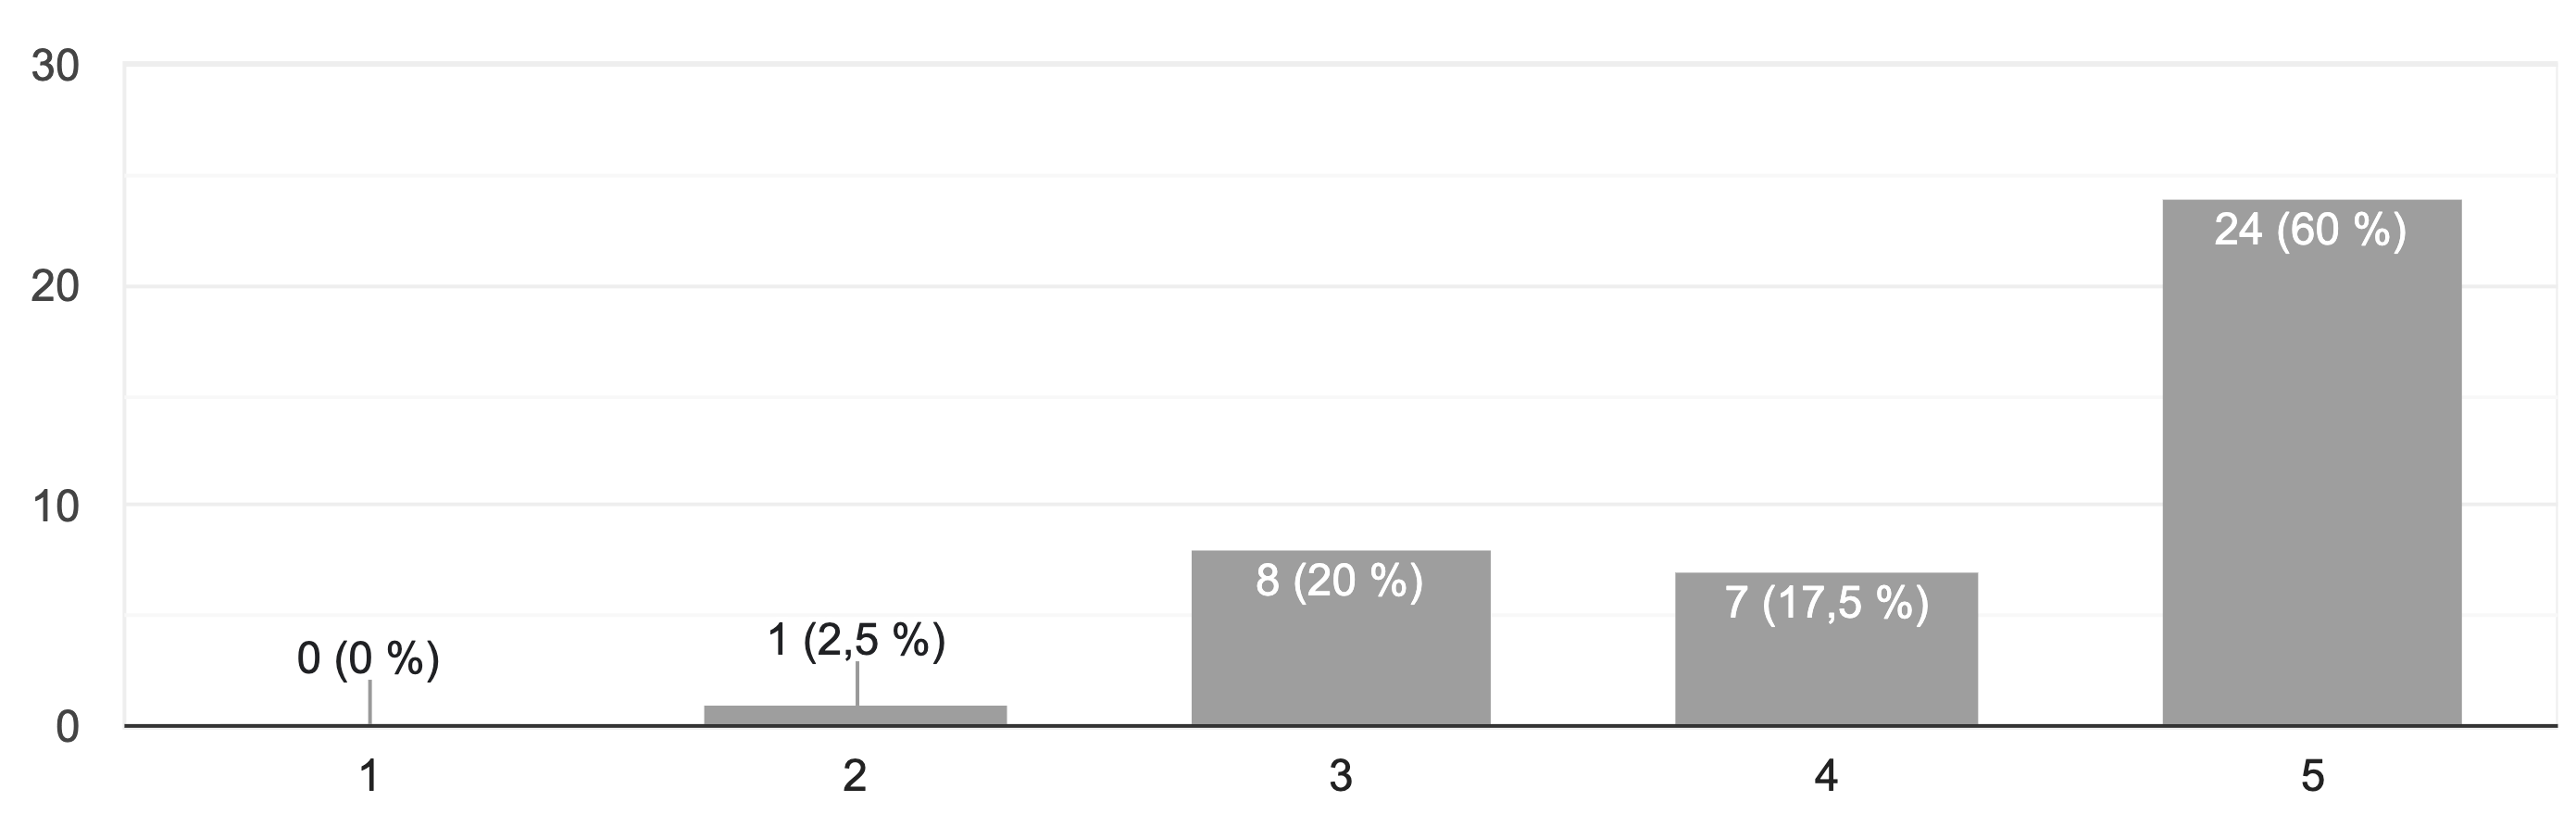
\includegraphics[width=\textwidth]{aufgabe_schwierigkeit_1}
    \caption{Wie schwer fandest du Aufgabe 1? (Auswertung Aufgabe 1)}
    \bildquelle{Google Forms}
    \label{fig:prototyp-umfrage-aufgabe-1-schwierigkeit}
\end{figure}

77,5 \% (31/40) der Befragten gaben an, dass die Aufgabe leicht zu bewältigen war (Schwierigkeitsstufe 4 oder 5). Aufgabe 2 war nach Einschätzung der Teilnehmenden wesentlich schwieriger als Aufgabe 1. Obwohl 70 \% angaben, dass die Aufgabe leicht zu bewältigen war, lag das Gewicht deutlich mehr auf Schwierigkeit 4 als auf Schwierigkeit 5 (siehe \autoref{fig:prototyp-umfrage-aufgabe-2-schwierigkeit}). Ferner ist der Anstieg bei der Schwierigkeitsstufe 2 (schwer) mit 15 \% signifikant. Bei dieser Einstufung hatte die vorherige Aufgabe im Vergleich nur einen Anteil von 2,5 \% mit einer Stimme. Im Verlauf wird diese Erkenntnis durch \autoref{table:prototyp-umfrage-aufgaben-schwierigkeit} mit den stochastischen Werten belegt.

\begin{figure}[H]
    \centering
    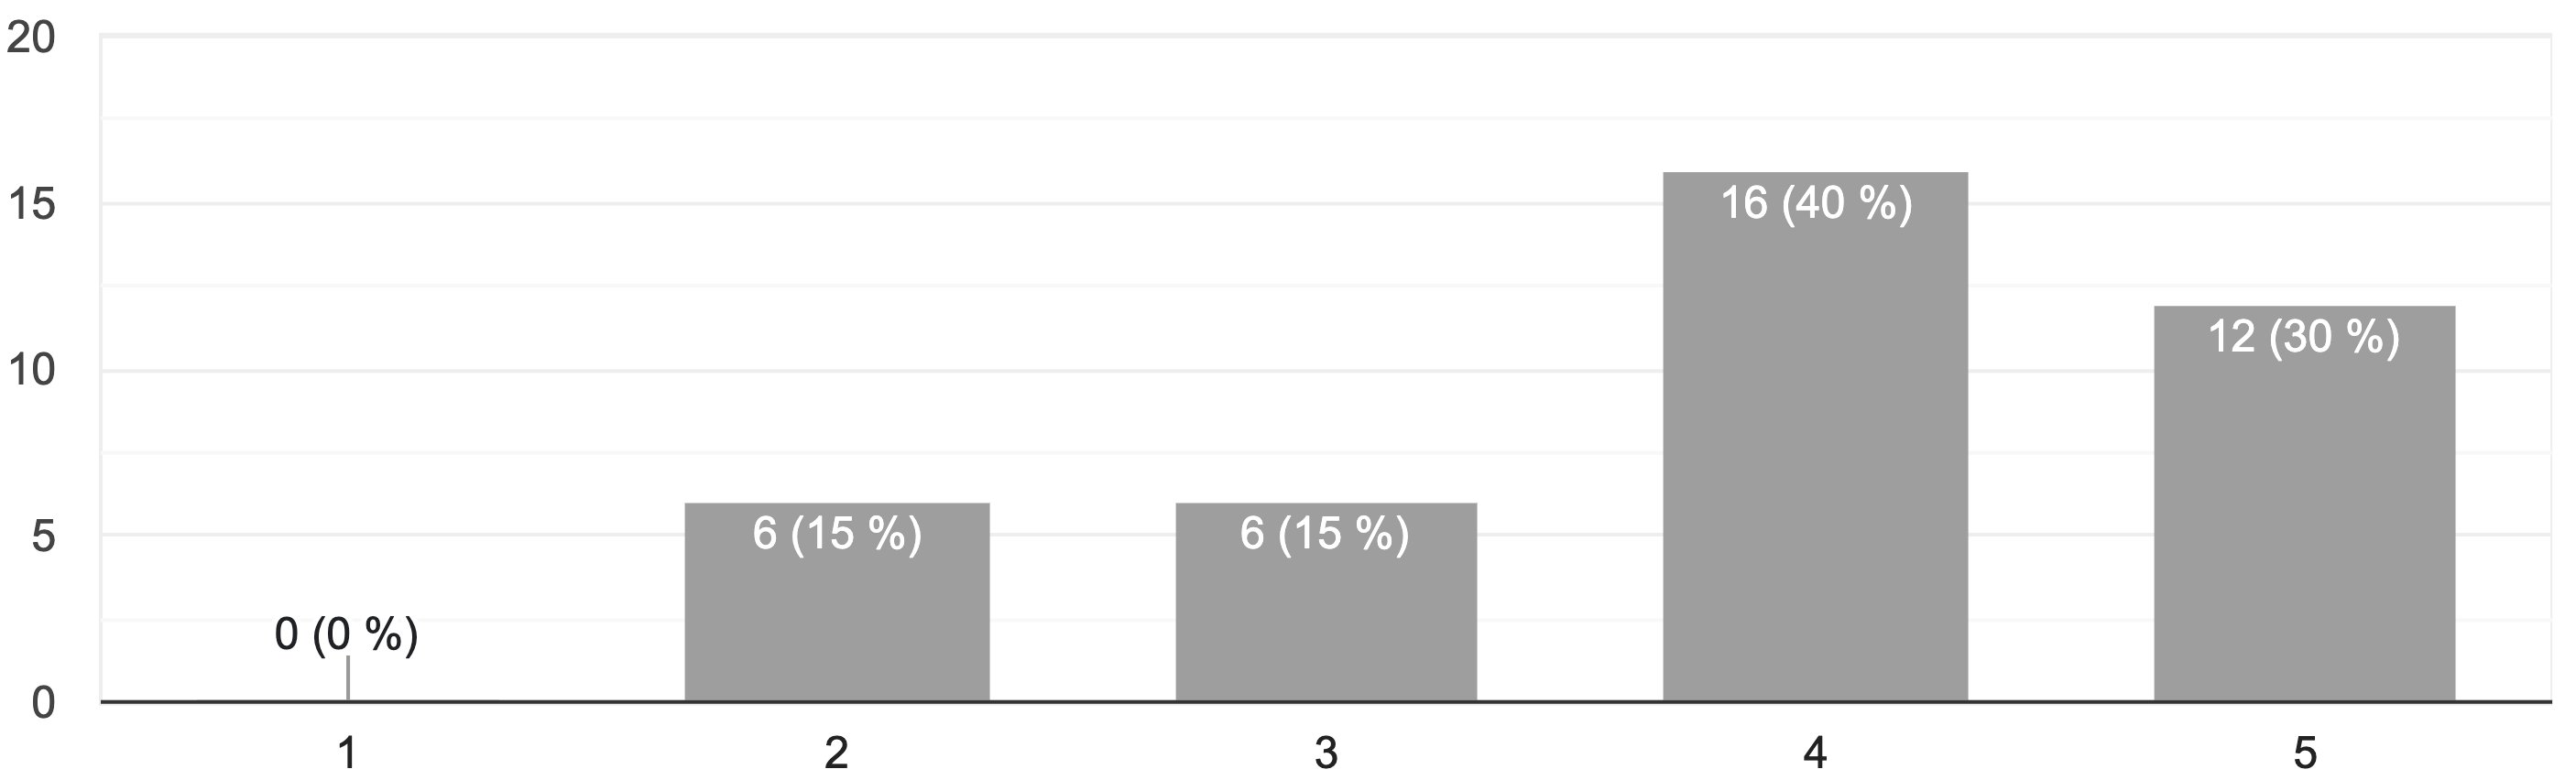
\includegraphics[width=\textwidth]{aufgabe_schwierigkeit_2}
    \caption{Wie schwer fandest du Aufgabe 2? (Auswertung Aufgabe 2)}
    \bildquelle{Google Forms}
    \label{fig:prototyp-umfrage-aufgabe-2-schwierigkeit}
\end{figure}

Zusammenfassend zeigt die stochastische Analyse in \autoref{table:prototyp-umfrage-aufgaben-schwierigkeit} die bereits aus den Diagrammen ersichtlichen Tendenzen. Sowohl der Durchschnitt als auch der Median sind bei Aufgabe 2 niedriger, was darauf hindeutet, dass diese als schwieriger empfunden wurde. Minimum und Maximum sind in beiden Aufgaben gleich. Das bedeutet, dass es bei beiden Aufgaben Befragte gab, die die Aufgaben als sehr leicht und als eher schwer empfanden. Keiner fand die Aufgaben jedoch unlösbar. Die Standardabweichung ist bei Aufgabe 2 höher als bei Aufgabe 1. Möglicherweise war Aufgabe 1 so einfach, dass viele Teilnehmer die richtige Lösung als selbstverständlich angesehen haben und deshalb der Großteil sehr einfach ankreuzen konnte. Bei Aufgabe 2 lag der Mittelwert eher in der Mitte der Skala, weshalb die Streuung höher ist und somit die Meinungen über die Schwierigkeit stärker differierten. 

\begin{table}[H]
    \renewcommand*{\arraystretch}{1.6}
    \centering
    \begin{tabular}{|l|l|l|l|l|l|} 
    \hline
    \diagbox{\textbf{Fragen}}{\textbf{Ergebnisse}} & \textbf{Durchschnitt} & \textbf{SD} & \textbf{Median} & \textbf{Min.} & \textbf{Max.}  \\ 
    \hline
    \textbf{Wie schwer fandest du Aufgabe 1?} & 4.350 & 0.882 & 5.000 & 2 & 5 \\
    \hline
    \textbf{Wie schwer fandest du Aufgabe 2?} & 3.850 & 1.014 & 4.000 & 2 & 5 \\ 
    \hline
    \end{tabular}

    \caption{Auswertung der Fragen zu den Aufgaben}
    \label{table:prototyp-umfrage-aufgaben-schwierigkeit}
\end{table}

\paragraph{Umfrage Teil 3: Aufgaben}

Der dritte Teil der Studie beinhaltet drei Fragen, die von den Schülerinnen und Schülern in Freitextfeldern beantwortet wurden.  Auch diese Felder werden mithilfe von Wordclouds ausgewertet, um schnell einen Überblick über die wichtigsten Punkte der Antworten zu erhalten.

% Was findest du am Konzept gut?

\begin{figure}[H]
    \centering
    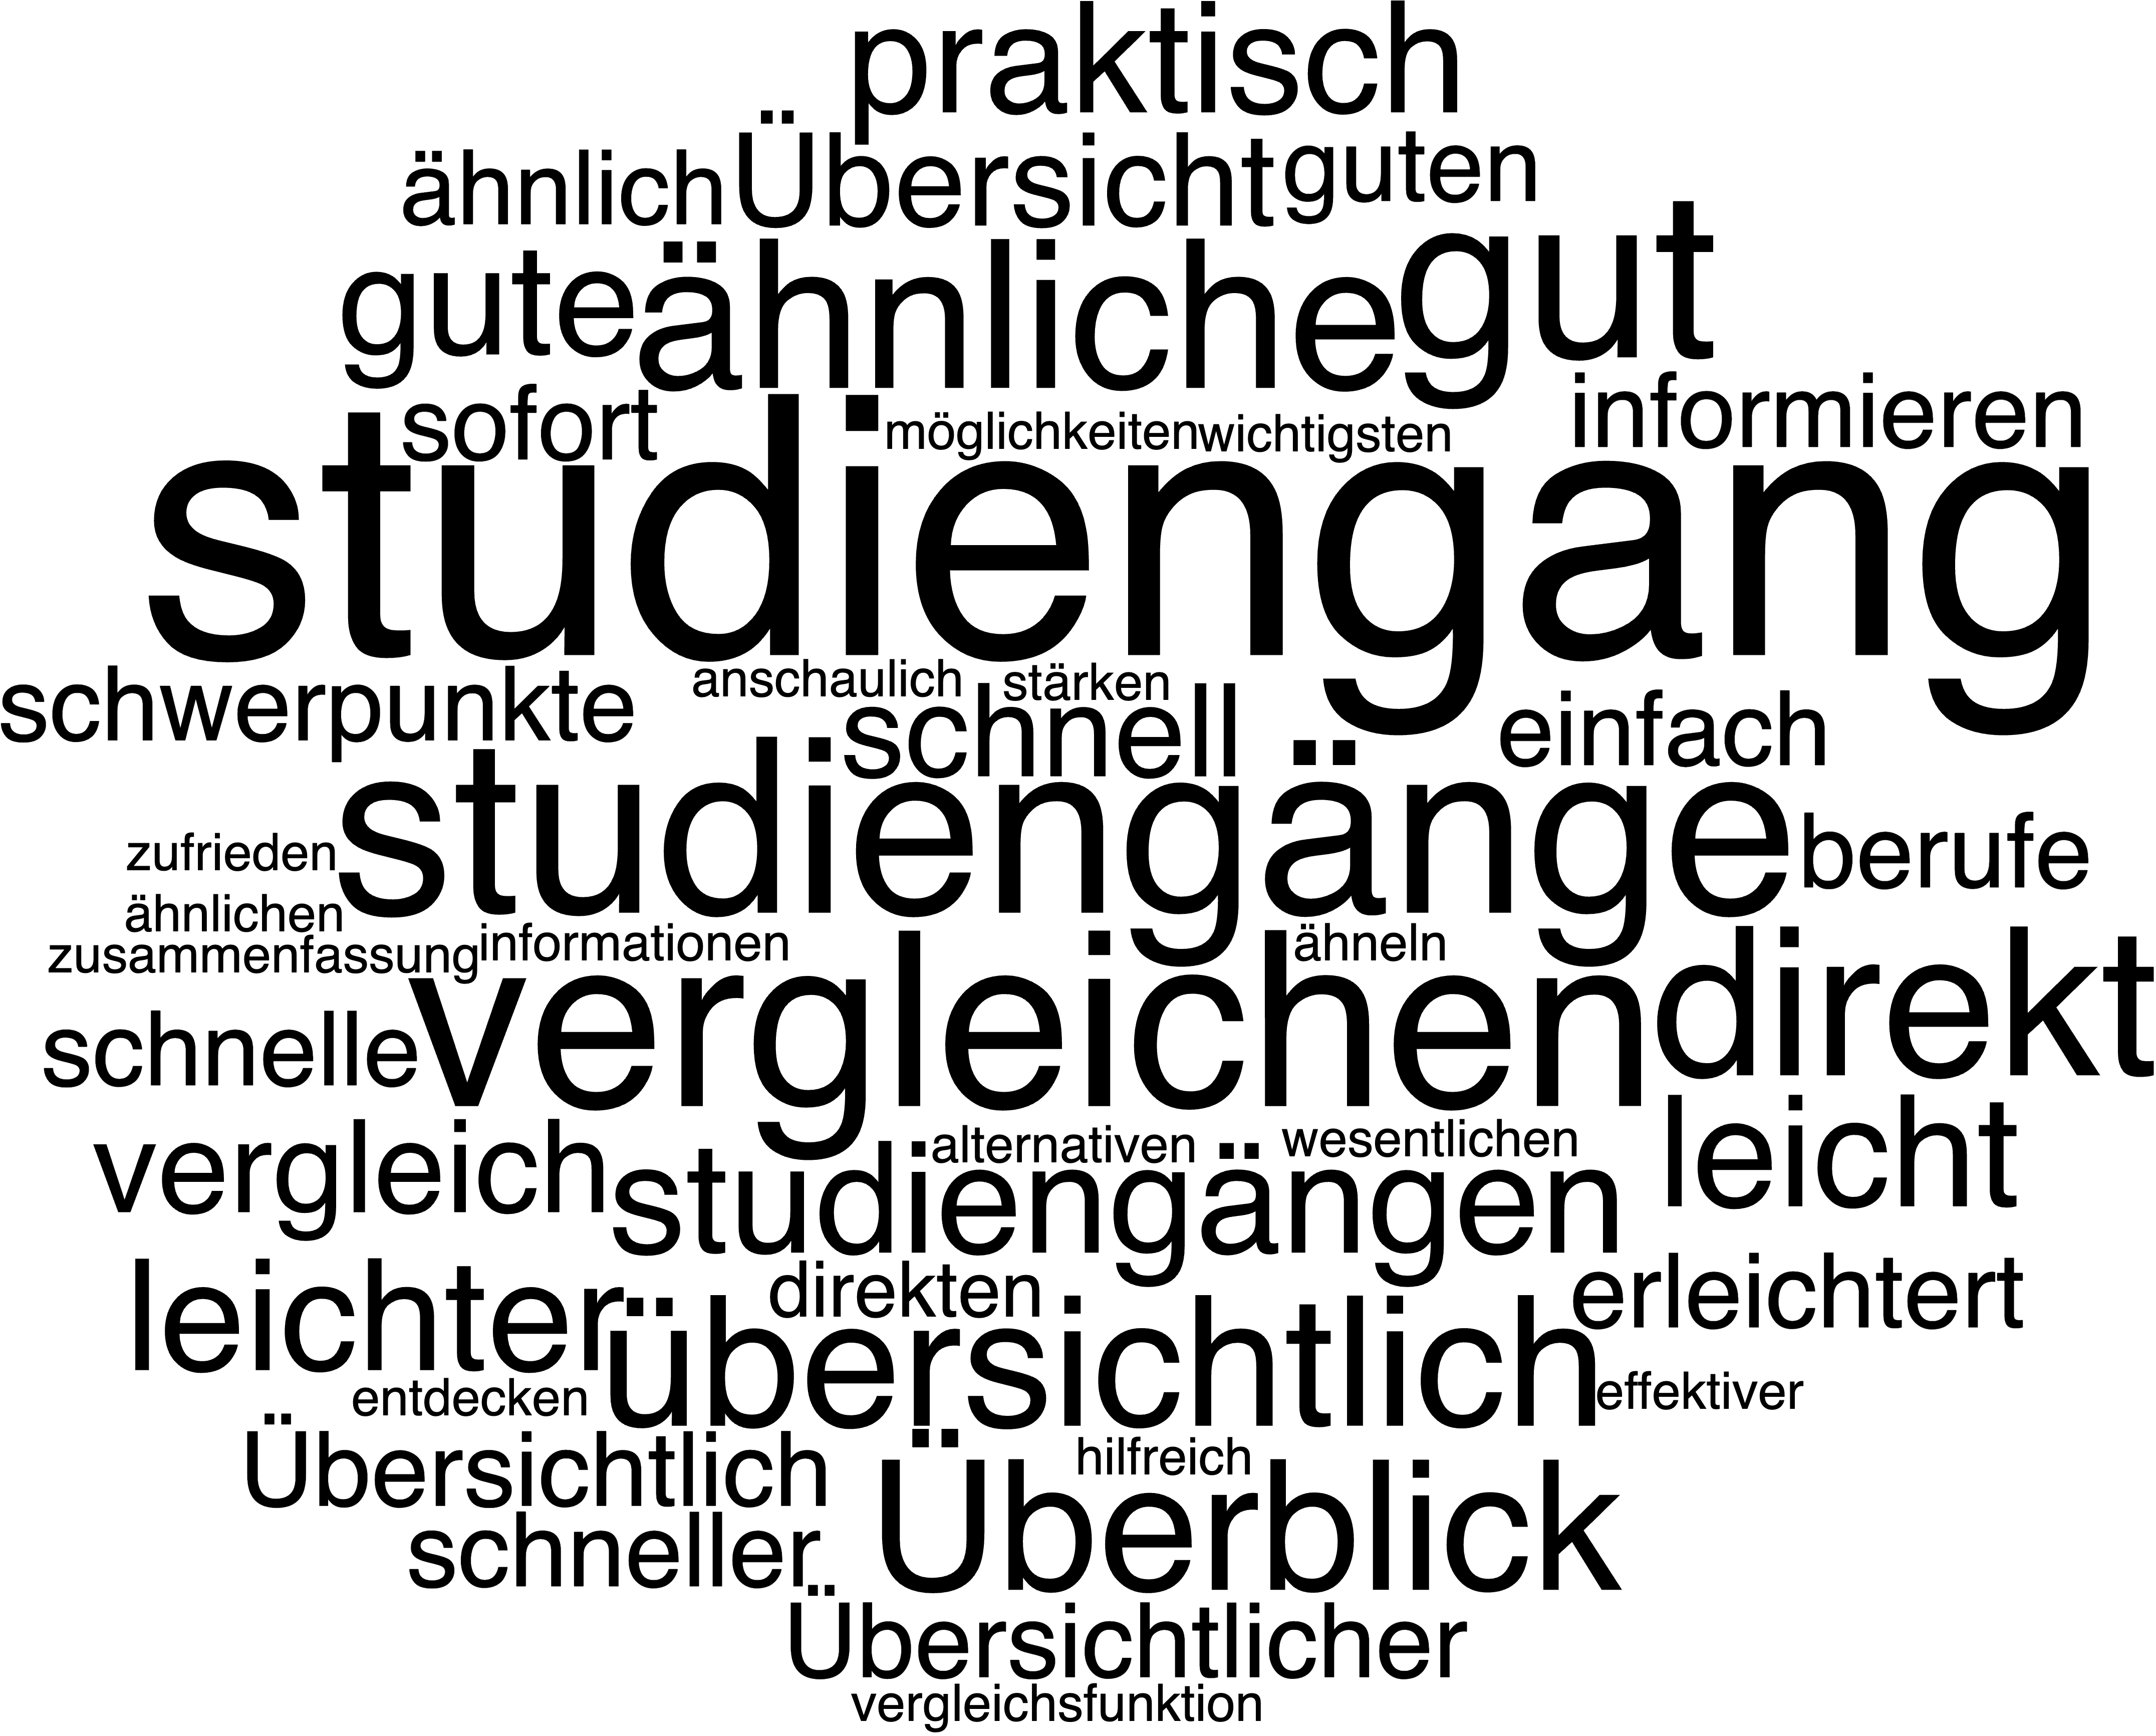
\includegraphics[width=0.6\textwidth]{aufgabe3.1-wordcloud}
    \caption{Wordcloud zu \glqq Was findest du an dem Konzept gut?\grqq{} (Umfrage Teil 3)}
    \bildquelle{Eigene Darstellung}
    \label{fig:prototyp-umfrage-aufgaben-3-1-wordcloud}
\end{figure}

\autoref{fig:prototyp-umfrage-aufgaben-3-1-wordcloud} zeigt die Wordcloud für die erste Frage des letzten Umfrageteils \glqq Was findest du an dem Konzept gut?\grqq{}. Wie bei der vorherigen Wortwolke sind häufig verwendete Begriffe prominenter (größer), während kleinere Begriffe nur selten verwendet wurden. Wie zuvor sind auch hier die vollständigen Antworten im Anhang zu finden. Ignoriert man die Begriffe \textit{Studiengang} und \textit{Studiengänge}, sind die Begriffe \textit{vergleichen} und \textit{Vergleich} mit insgesamt 20 Vorkommnissen sehr präsent. Es lässt sich schlussfolgern, dass die Implementierung der Vergleichsfunktion in den Prototypen erfolgreich ist und weiterverfolgt und optimiert werden sollte.

Weitere Schlagwörter, die ins Auge fallen, sind \textit{schnell}, \textit{übersichtlich}, \textit{Überblick}, \textit{direkt}, \textit{leicht}, \textit{praktisch} und \textit{ähnliche}. Diese Begriffe beziehen sich möglicherweise auf das allgemeine Konzept des Studiengangsfinders und unterstützen erneut die Basis des Konzepts, dass eine solche Art von Software bei der Studiengangsfindung für Studieninteressierte sehr nützlich sein kann.

% Was findest du am Konzept schlecht?

\begin{figure}[H]
    \centering
    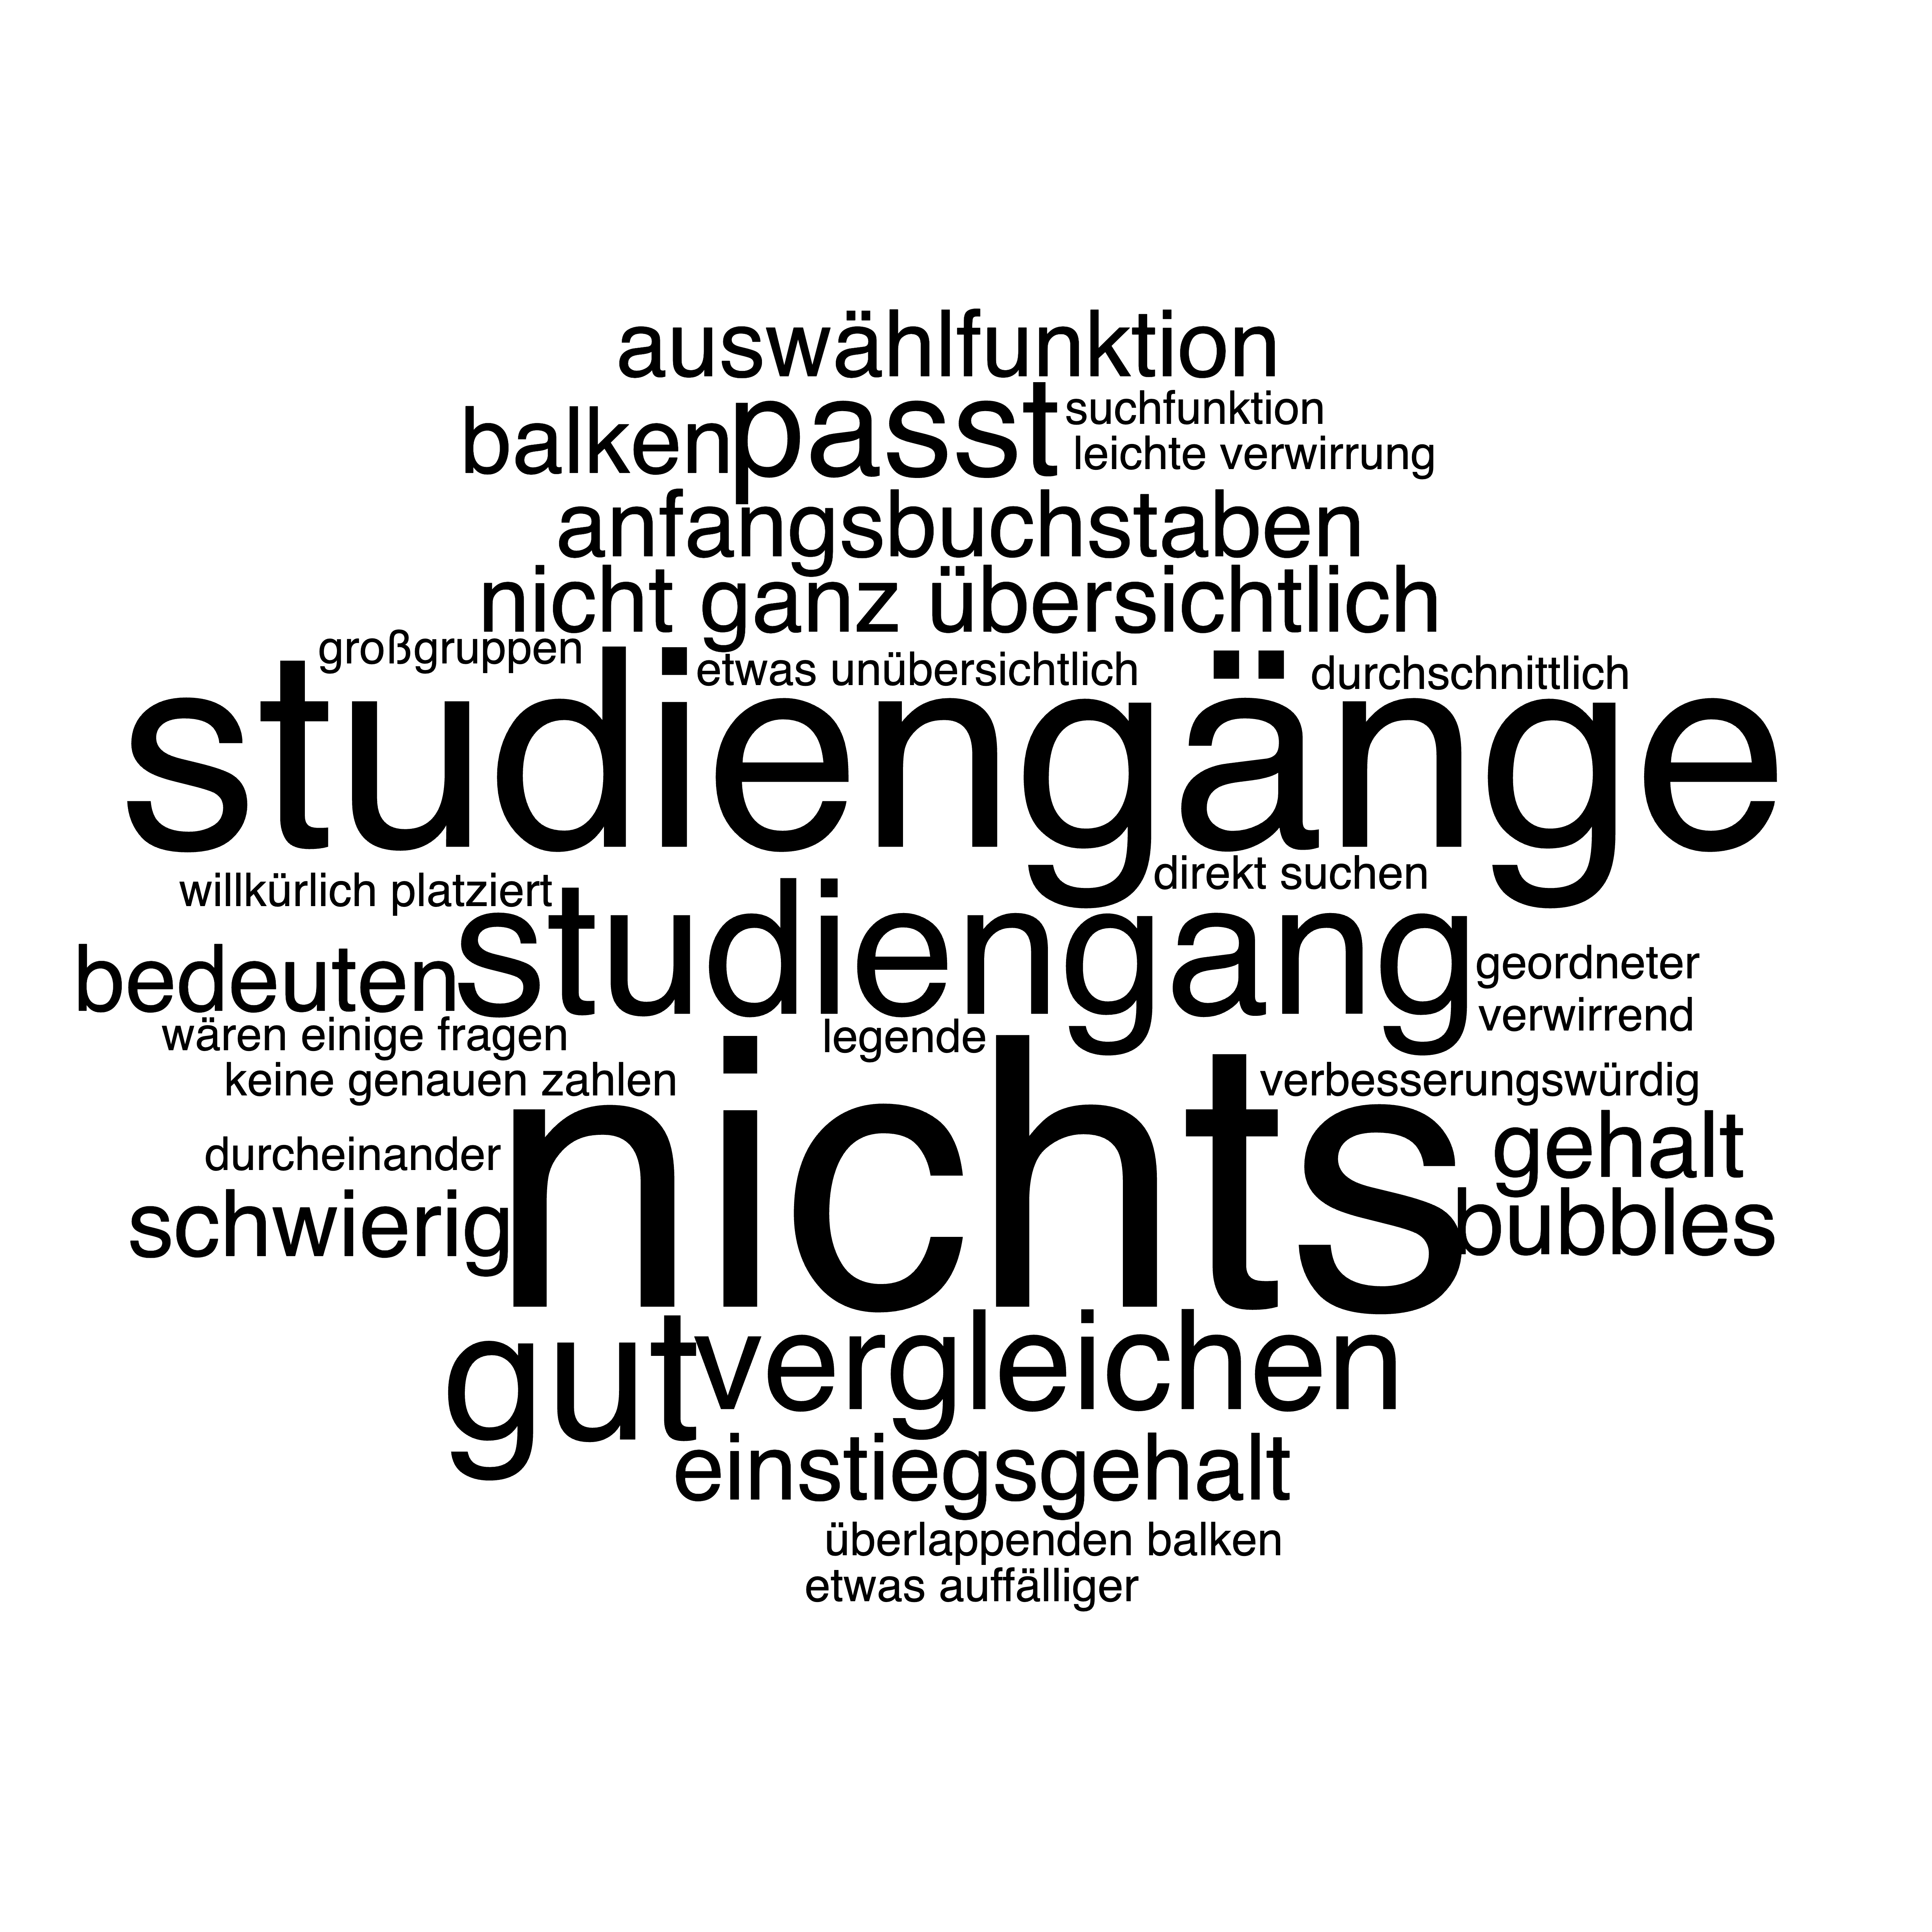
\includegraphics[width=0.6\textwidth]{aufgabe3.2-wordcloud}
    \caption{Wordcloud zu \glqq Was findest du an dem Konzept schlecht?\grqq{} (Umfrage Teil 3)}
    \bildquelle{Eigene Darstellung}
    \label{fig:prototyp-umfrage-aufgaben-3-2-wordcloud}
\end{figure}

Die zweite Frage lautete: \glqq Was findest du am Konzept schlecht?\grqq{}. Für diese Frage wurde ebenfalls eine Wordcloud erstellt (siehe \autoref{fig:prototyp-umfrage-aufgaben-3-2-wordcloud}). Um alle Punkte vollständig zu erfassen, wurde jedoch hauptsächlich mit den Original-Antworten gearbeitet. Der am häufigsten genannte Begriff in Bezug auf die Zufriedenheit war \textit{nichts}. Das bedeutet, dass die Mehrheit bereits mit dem Prototyp zufrieden war. Allerdings lassen sich bei genauerer Betrachtung einige Kritikpunkte feststellen:

\begin{itemize}
    \item Übersichtlichkeit bei vielen Bubbles
    \item Platzierung von Bubbles wirkt willkürlich
    \item Beim Vergleich ist nicht klar erkennbar, welche Farbe dem ursprünglich ausgewählten Studiengang und welche dem Vergleichsstudiengang zugeordnet ist
    \item In der Funktion \glqq Studiengang vergleichen\grqq{} sollten die Studiengänge entweder alphabetisch sortiert oder durch eine Suchfunktion filterbar sein.
    \item Legende für direkten Vergleich einfügen
    \item Die Vergleichsoption sollte auffälliger gestaltet werden
    \item Was passiert, wenn ein Studiengang inhaltlich in zwei übergeordnete Gruppen fällt?
    \item Erforderliche Soft Skills mit angeben
    \item Button \glqq Mehr erfahren\grqq{} geht in der Übersicht unter
    \item Einstiegsgehalt in absoluten Zahlen
\end{itemize}

Zusammenfassend sollte die Platzierung der Bubbles erklärt werden. Diese erfolgt nicht willkürlich, sondern mithilfe des MDS-Algorithmus und der Inhalte des Studiengangs automatisch. Im Endprodukt werden die Bubbles voraussichtlich durch einen bereinigten und vollständigen Datensatz besser platziert sein, wodurch sich dieser Kritikpunkt beheben lassen wird.

Die Farbe des Vergleichsfeatures wurde mehrmals kritisiert. Zum Zeitpunkt der Studie werden die Inhaltsbalken des zu vergleichenden Studiengangs mit einem neutralen Grau über die des original angeklickten Studiengangs gelegt. Eine mögliche Verbesserung wäre die Verwendung einer Farbänderung, eines zusätzlichen Hilfe-Dialogs oder einer Legende. Um eine schnellere Suche zu ermöglichen, könnten die zu vergleichenden Studiengänge vor der Auslieferung ans Frontend durch das Backend alphabetisch sortiert werden.

Ferner ist es kein Hindernis, wenn ein Studiengang inhaltlich in zwei Gruppen fällt, da immer der höchste Wert zur Gruppenzugehörigkeit gewählt wird. Wenn zwei Kategorien denselben Wert haben und gleichzeitig die höchsten Werte sind, wird die erste Kategorie verwendet. Außerdem ist es kein Problem, da die Wahrscheinlichkeit hoch ist, dass die Bubbles nahe beieinander liegen, wenn der Algorithmus berechnet wird. Selbst wenn sie sich in verschiedenen Supergruppen befinden, werden sie aufgrund ihrer Koordinaten als ähnliche Studiengänge betrachtet.

Es gestaltet sich eher schwierig, erforderliche Soft Skills für das Studium anzugeben, da es keine offizielle und einheitliche Dokumentation über die benötigten Soft Skills pro Studiengang gibt.

Der Button \glqq Mehr erfahren\grqq{} geht in der Übersicht unter. Dieser Punkt wurde von nur einer Person geschrieben und die Schaltfläche ist im Vergleich zu den anderen Elementen bereits sehr groß und deutlich sichtbar. Sie befindet sich auf der rechten Seite der Aktionsleiste. Aus diesem Grund wird der Kritikpunkt nicht weiter evaluiert.

Es wurde zweimal nach dem Einstiegsgehalt in konkreten Zahlen gefragt. Ein Nachteil dieser Implementierung besteht darin, dass die Werte regelmäßig überprüft und gewartet werden müssen, im Gegensatz zur aktuellen Implementierung mit den einfachen Bewertungen \glqq Überdurchschnittlich\grqq{}, \glqq Durchschnittlich\grqq{} usw. Deshalb wird dieser Punkt auch nicht weiter untersucht.

% Hast du neue Ideen für den Prototypen?
% Text: Auch hier muss mit den ganzen Antworten gearbeitet werden
\begin{figure}[H]
    \centering
    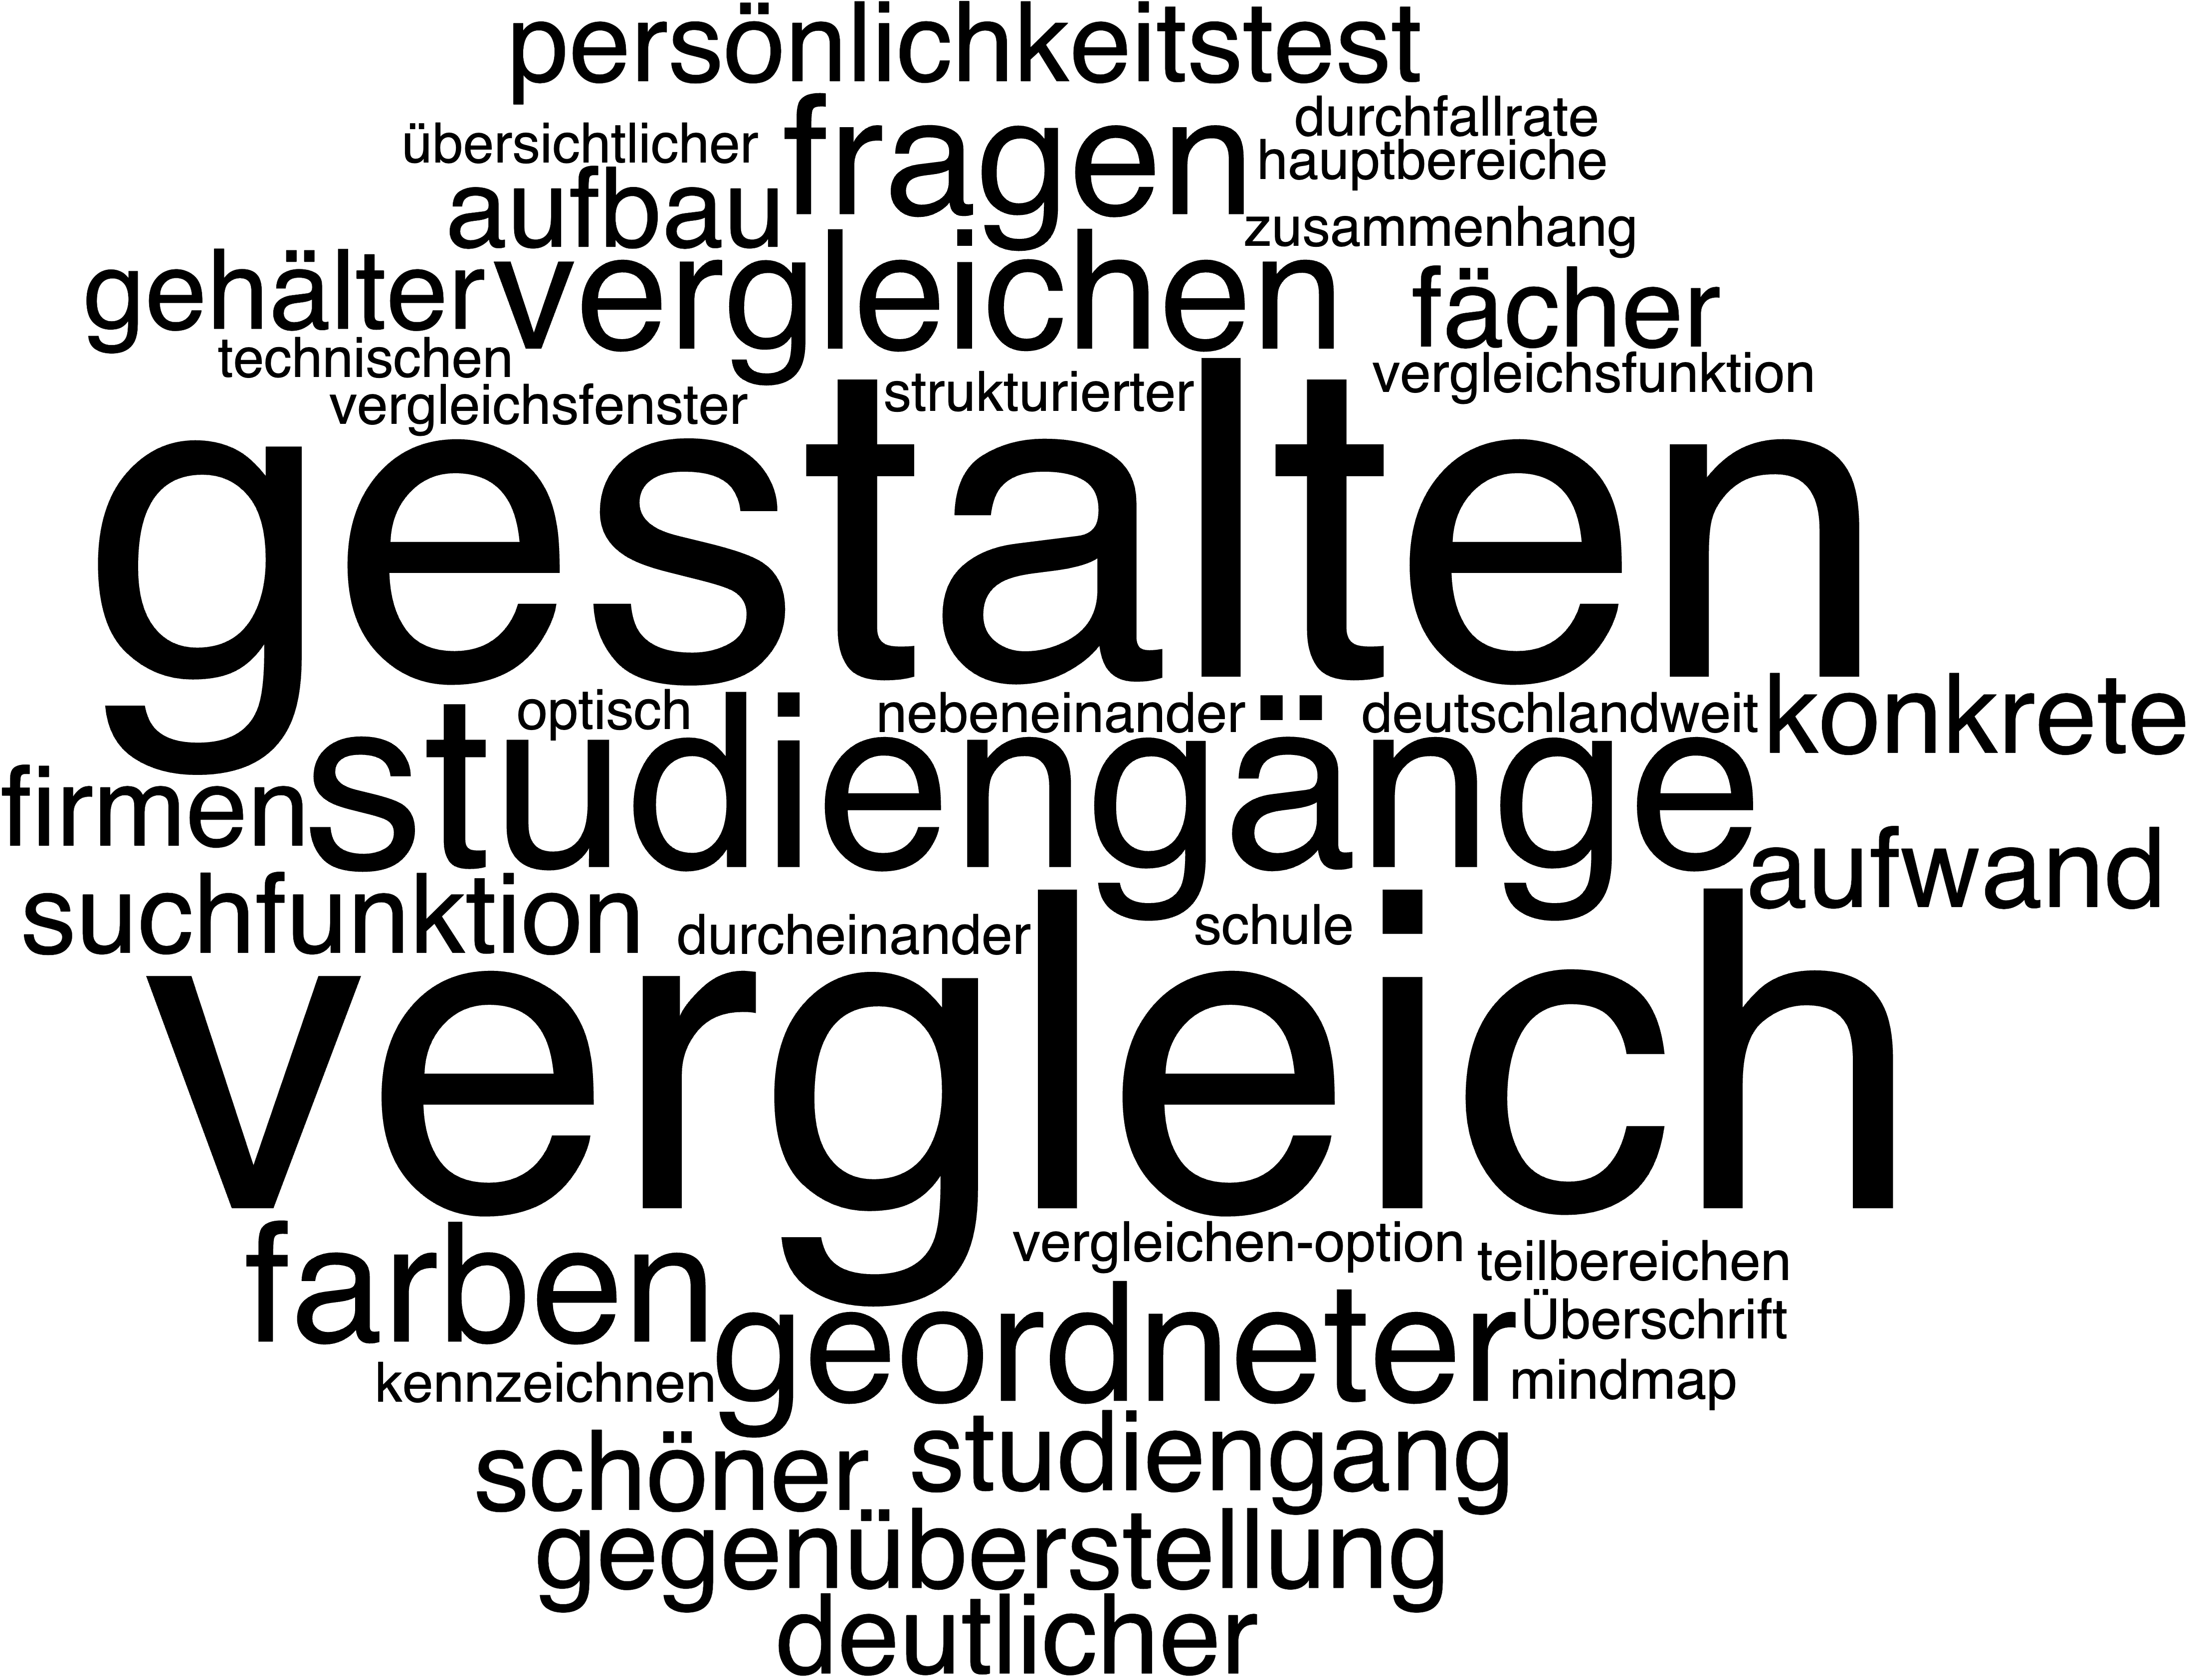
\includegraphics[width=0.6\textwidth]{aufgabe3.3-wordcloud}
    \caption{Wordcloud zu \glqq Hast du neue Ideen für den Prototypen?\grqq{} (Umfrage Teil 3)}
    \bildquelle{Eigene Darstellung}
    \label{fig:prototyp-umfrage-aufgaben-3-3-wordcloud}
\end{figure}

Die in \autoref{fig:prototyp-umfrage-aufgaben-3-3-wordcloud} genannten Punkte ähneln sehr den Kritikpunkten, die in der vorherigen Frage \glqq Was findest du an dem Konzept schlecht?\grqq{} behandelt wurden. Im Folgenden werden die Kritikpunkte auf Basis der Wordcloud und den vollen Antworten der Teilnehmenden gruppiert und zusammengefasst dargestellt. Die Original-Antworten sind, wie bei den vorherigen Fragen auch, im Anhang aufgeführt.


\begin{itemize}
    \item Vergleichsfunktion optisch ansprechender gestalten
    \item Vergleichsfunktion über mehr als zwei Studiengänge
    \item Suchfunktion zur Vergleichsfunktion hinzufügen
    \item Persönlichkeitstest einführen (als Orientierung)
    \item Ähnliche Studiengänge anders platzieren/gestalten
    \item Absolute Werte bei Gehälter
    \item Mehr Informationen zu den einzelnen Fächern ggf. Bezug auf die Schule
    nehmen
    \item Farben ändern
\end{itemize}
%% Punkte einfügen

Die optische Gestaltung der Vergleichsfunktion wurde mehrmals erwähnt. Die Farben und die Gestaltung des Buttons zur Aktivierung der Vergleichsfunktion sowie der Inhaltsbalken sollten geändert werden. Außerdem wurde der Wunsch geäußert, dass man mehr als zwei Studiengänge gleichzeitig vergleichen kann. Es stellt sich jedoch die Frage, ob dies sinnvoll ist, da es auf mobilen Endgeräten schnell unübersichtlich werden könnte. Ein weiterer oft genannter Wunsch ist eine Suchfunktion innerhalb der Vergleichsfunktion. Wie schon bei der vorhergehenden Frage beschrieben, könnte hier entweder eine alphabetisch sortierte Liste oder ein Textfeld mit automatischer Vervollständigung verwendet werden. Ein Autocomplete-Textfeld schlägt Vorschläge vor, während Buchstaben eingegeben werden. Es ähnelt somit einem Suchfeld.

Außerdem wurde mehrfach ein Persönlichkeitstest gewünscht, der spezifische Fragen an den oder die Studieninteressierte stellt und daraus eine Empfehlung für das zu wählende Studium ableitet. Wie bereits in \autoref{sec:konzepte-von-studiengangsfindern} erwähnt, bringt dies jedoch auch einige Limitierungen mit sich. Eine Möglichkeit für die Zukunft wäre, eine optionale Online-Umfrage anzubieten. Diese könnte die Ergebnisse aufgrund der eingegebenen Daten in StudyMap als eine Art Heatmap darstellen und die Zugehörigkeit zu einer bestimmten Position und somit zu einer Supergruppe bzw. Studiengang markieren. Eine Heatmap ist eine grafische Darstellung von Daten, bei der Werte in einer Matrix durch Farben codiert werden. Intensivere Farben repräsentieren höhere Werte, um Muster oder Trends visuell hervorzuheben. In diesem Fall werden die Zugehörigkeiten zur Kategorie \glqq Wirtschaft\grqq{} dargestellt. 

Es wurde erwähnt, dass die Sektion \glqq Ähnliche Bachelor-Studiengänge\grqq{} nicht gut platziert ist. Dieser Eindruck könnte aufgrund der eher standardmäßigen Gestaltung (siehe \autoref{fig:mockup-bubbles-popup} ganz unten im Popup) entstehen. Eine Möglichkeit wäre, die Studiengänge mit Icons zu versehen oder sie wie bei dem Abschnitt \glqq Firmen in Regensburg\grqq{} mit schwarzen, abgerundeten Rechtecken als Schaltflächen zu präsentieren.

Absolute Werte bei den Gehältern können aus den vorher genannten Gründen nicht umgesetzt werden.

Für die Kurzübersicht wäre es vermutlich zu umfangreich, Informationen zu den einzelnen Fächern bereitzustellen. Das Popup ist bereits sehr voll - mehr Inhalt könnte die Benutzererfahrung negativ beeinflussen. Ein zusätzlicher Reiter für alle Fächer wäre vermutlich zu viel. Um die einzelnen Fächer einzusehen, muss der Interessierte lediglich auf den Button \glqq Mehr erfahren\grqq{} klicken und schließlich den Studienverlaufsplan des jeweiligen Studiengangs öffnen. Dort sind alle präzisen Informationen über den Studiengang für den Benutzer zu finden. StudyMap bietet einen Überblick und eine grobe Orientierungshilfe für das Studium. Für weitere Informationen steht Studieninteressierten die OTH-Website mit detaillierten Informationen zu allen Studiengängen zur Verfügung.

Wie bereits in \autoref{sec:visualisierung-der-studiengänge} erläutert, werden die Bubbles in den Fakultätsfarben eingefärbt. Dies ist eine Anforderung der Vizepräsidentin der OTH-Regensburg und der Fakultäten der Hochschule. Daher kann dem Wunsch nach anderen Farben nicht entsprochen werden. Andere Farben könnten zu Verwirrung führen, da nicht klar ist, warum eine bestimmte Bubble beispielsweise grün gefärbt ist. Die aktuelle Lösung definiert klar, welcher Studiengang welche Farbe erhält. So umfasst z.B. die Supergruppe Technik nicht nur die Studiengänge der Fakultät Maschinenbau, sondern auch die Studiengänge der Fakultät für Elektro- und Informationstechnik. Obwohl die Studiengänge in derselben Supergruppe sind, kann man sie durch die Farben leichter voneinander unterscheiden.

\subsection{Zusammenfassung der Studien}
Zusammenfassend wurde durch die Anwendung der Mockup-Studie ein positiv bewertetes Konzept für den Prototypen entwickelt. Durch den Prozess des User Centered Designs wurden die späteren Benutzer von Anfang an in den Entwicklungsprozess einbezogen. Dadurch wird sichergestellt, dass die Bedürfnisse der Zielgruppe im finalen Produkt möglichst umfassend erfüllt werden.

Da die Anforderungen der Zielgruppe von Anfang an klar definiert sind, kann durch den Einsatz von UCD die Entwicklungszeit deutlich verkürzt werden. Beide Studien erzielten ähnliche Ergebnisse. Der Hauptkritikpunkt an den Entwürfen bzw. dem Prototypen ist die mangelnde Übersichtlichkeit. Zusammenfassend lässt sich festhalten, dass alle Teile des Endprodukts durch Hilfedialoge erläutert werden sollten. Es muss auch geprüft werden, ob eine Legende für die Bubbles als Erklärung erforderlich ist. Der Fokus sollte also auf der Darstellung von möglichst vielen Informationen in möglichst übersichtlicher Form liegen, um den Nutzern einen Überblick und Vergleich aller Studiengänge zu ermöglichen.

Durch die erste Mockup-Studie konnten bereits einige Schwachstellen des Entwurfs behoben werden, die bei der Implementierung des Prototypen berücksichtigt wurden. Bereits in dieser Phase konnte Entwicklungszeit eingespart werden, da Änderungen mithilfe des Mockups vor der ersten Entwicklung geplant werden konnten. Das positive Feedback auf den Prototyp im Rahmen der Prototypenstudie von 37 Studieninteressierten war eine Bestätigung für den Bedarf an StudyMap als Instrument zur Studienorientierung.

Zusammenfassend ist festzuhalten, dass die Studien erfolgreich verlaufen sind. Als Ausblick in die Zukunft könnte ein Orientierungstest interessant sein. Dieser Test würde den Studierenden anhand einiger Fragen eine Position auf der StudyMap zuweisen, damit sie sich die Studiengänge in der Nähe dieser Position genauer ansehen können. Eine weitere Idee für die Zukunft ist, dass mehr als nur zwei Studiengänge inhaltlich miteinander verglichen werden können.